\documentclass{article}

\usepackage[T1]{fontenc}
\usepackage[french]{babel}
\usepackage[a4paper, margin=1.5cm]{geometry}
\usepackage{graphicx}
\usepackage[colorlinks = true, allcolors = blue]{hyperref}
\usepackage{float}

\graphicspath{ {./images/} }

\begin{document}

\begin{titlepage}

\begin{center}
    \begin{minipage}{10cm}
        \begin{center}
        \textbf{UNIVERSITE DE BORDEAUX}\\[0.1cm]
        \end{center}
    \end{minipage}

{\huge \bfseries \uppercase{Projet De Programmation} \\[0.5cm] }

\rule{\linewidth}{0.3mm} \\[0.4cm]
{ \huge \bfseries\color{blue} Hex - Python \\[0.4cm] }
\rule{\linewidth}{0.3mm} \\[3cm]

\noindent
\begin{minipage}{.25\textwidth}
  \begin{flushleft} \large
    \textbf{M.}~\textsc{KUSTERS} Timon\\
    \textbf{M.}~\textsc{HERR} Mariano\\
    \textbf{M.}~\textsc{HUBINCU} Morgan\\
    \textbf{M.}~\textsc{ROCHETEAU} Yohann\\
    \textbf{M.}~\textsc{GUITARD} Paul\\
  \end{flushleft}
\end{minipage}%
\begin{minipage}{0.5\textwidth}
  
\end{minipage}\\[1cm]

\vfill
{\textbf{\large {Année universitaire} 2024-2025}}

\end{center}
\end{titlepage}

\newpage

\tableofcontents

\newpage
\section{Présentation du projet}

\subsection{Règles du jeu}

Le jeu de Hex est un jeu de plateau se basant sur de la stratégie, sans notion de hasard ou de chance. Une partie se joue sur un plateau en forme de losange régulier (carré), remplis de cases hexagonales. La partie se joue à deux joueurs, ayant pour l'un des pions blancs et pour l'autre des pions noirs. Chaque joueur se voit attribuer deux bordures parallèles du plateau. Le but du jeu est de les connecter via une ligne de pions hexagonaux contigus de sa propre couleur, en plaçant un pion chacun à son tour sur n'importe quelle case, à la seule condition que cette dernière soit libre. Selon le théorème de Nash (\cite{VVA2002}), le match nul n'existe pas, un joueur parvient toujours à joindre ses deux bordures de plateau avant que celui-ci ne soit complètement rempli.

\begin{figure}[H]
    \centering
    
\includegraphics[width=0.75\linewidth]{hex.png}
    \caption{Image montrant une partie de Hex gagnée par le joueur ayant les pions bleus.}
    \label{fig:hex}
\end{figure}

\subsection{Existant du projet}

Faisant uniquement appel à la logique, le jeu de Hex est un bon problème pour tester et développer des algorithmes de recherche et leurs heuristiques en IA. De nombreux papiers présentent des méthodes, des outils et des approches manipulant ce jeu. Des compétitions entre plusieurs joueurs artificiels ont eu lieu, comparant les efficacités des algorithmes des compétiteurs. C'est le cas des outils MoHex \cite{AHH10} et Yopt \cite{CS08} qui implémentent la recherche arborescente Monte-Carlo. Quelques heuristiques y sont discutées. Un article en compile quelques-unes \cite{RJ02}. Ces informations nous seront utiles lors de l'implémentation du joueur artificielle.

En ce qui concerne le jeu de base, le plateau est souvent implémenté à l'aide de tableau en deux dimensions \cite{playhex} ou par un graphe \cite{JAhex} ou par une structure permettant l'union rapide pondérée \cite{Abdo}. Le plateau du jeu de Hex peut aussi, comme de nombreux autres jeux comme le Go ou les échecs, être représenté par des bitboards. Des méthodes communes à ces jeux ont été créées et explicitées par Browne \cite{browne14} dont une qui permet la détection de connexions qui marque la fin de partie dans le jeu de Hex. L'algorithme présenté, le bitwise-parallel reduction \cite{browne12}, utilise une Y-réduction (expliquée plus tard \ref{yreduction}) qui est une structure qui peut être obtenue à partir de bitboards et permet des opérations parallèles entre les colonnes du plateau. Ces différents algorithmes, projets et articles pourront être repris, adaptés ou servir d'inspiration lors de l'implémentation de nos besoins les plus complexes.

\subsection{Principaux algorithmes et structures utilisés}

\subsubsection{Structures}

\begin{enumerate}
    \item État du jeu : 
        \begin{itemize}
            \item Cette structure est en 5 parties :
            \begin{itemize}
                \item Le joueur courant (entier), le tour actuel (entier) et l'état du plateau (deux bitboards)
                \item Les historiques de coups joués
                \item Les temps restants des joueurs en mode blitz
                \item La configuration du jeu (On stocke dans cette structure les options passées en arguments ainsi que les paramètres lus depuis le fichier de configuration)
            \end{itemize}
        \end{itemize}
    \item Bitboard :
        \begin{itemize}
            \item Le plateau de jeu sera stocké sous la forme de plusieurs bitboards, des mots binaires. Ces bitboards auront une taille égale au nombre de cases du plateau. Un bit représentera une case. Ces bitboards seront implémentés par la structure bitarray du module homonyme. Ce sont des mots binaires ayant une taille dynamique qui permettent les opérations sur bits telles que |, \&, <<, etc. Leur utilisation est plus rapide que les $long$ en python qui ont aussi une taille dynamique. Cette structure présente plusieurs avantages par rapport à un tableau en deux dimensions ou un graphe :
            \begin{itemize}
                \item Usage de la mémoire : un ou plusieurs entiers pour un plateau entier au lieu d’un entier par case.
                \item Lectures et écritures efficaces grâce aux opérations sur bits.
                \item Calcul vectorisé : les opérations se font sur toutes les cases en même temps.
            \end{itemize}
            Pour représenter le plateau, on utilisera deux bitboards : 
            \begin{itemize}
                \item bitboard pour les pièces blanches $bits_w$
                \item bitboard pour les pièces noires $bits_b$
            \end{itemize}
        \end{itemize}
    \item Historiques des coups joués :
        \begin{itemize}
            \item On utilise une structure de type FIFO pour représenter les historiques de coups. L'ajout, la suppression et la lecture de l'élément en tête se faisant en temps constant, cette structure est efficace, car nos opérations (revenir en arrière d'un coup, revenir vers l'avant) ne manipulent, le plus souvent, seulement cet élément en tête. Deux FIFO manipulant des triplets \textit{(nombre\_du\_tour, joueur, coup)} correspondant respectivement à l'historique des coups joués et l'historique des coups annulés serviront à naviguer entre les coups. Elles seront implémentées par la structure deque du module collections.deque, car cela sera plus simple de parcourir la structure pour l'affichage de l'historique. 
        \end{itemize}
\end{enumerate}

\subsubsection{Algorithmes}

\begin{enumerate}
    \item Bitboards :
        \begin{itemize} \label{bitalgo}
            \item Savoir si un coup est légal : $\lnot( bits_w | bits_b)$ donne le bitboard des cases vides (bit à 1 == case vide). On compare ensuite ce bitboard avec le coup joué pour voir si coup légal (exemple : blanc veut jouer en "d1". "d1" traduit en position dans le bitarray devient 4 et la formule $(bits_w >> 4) \;\&\; 1$ est égale à 1 si la case est occupée et 0 si elle est vide).
            \item Jouer un coup : Si blanc joue "d1" il suffit de faire $bits_w = bits_w\;|\;4$
            \item Détecter une connexion : On utilise une Y-réduction comme \cite{browne12}. Dans cette structure, le plateau est représenté par un entier pour chaque colonne et les cases du plateau sont représentées par une paire de bits. “00” pour une case vide, “01” pour une case blanche, “10” pour une case noire, “11” pour les cases inutilisées. Cette méthode fait perdre un peu d’espace mémoire (on passe de 2 entiers à $dim+1$ entiers, $dim$ étant une dimension du plateau du jeu, par exemple 13 dans un jeu de hex de taille 13x13) mais on garde les opérations sur bit. La détection se fera comme ceci :
            \begin{enumerate}
             \label{yreduction}
                \item On convertit les bitboards en une Y-réduction. Pour cela, on parcourt les bits des 2 bitboards en ajoutant, si le bit d’un des 2 bitboards est à 1, 2 bits comme le codage ci-dessus à la position $2^{(2\times i)}$. Les bitboards sont parcourus par ligne donc on construit deux bits de chaque colonne toutes les $dim$ tours de boucles. On ajoute une autre colonne en plus des $dim$ colonnes ainsi que 2 bits en plus pour chaque colonne qui vont représenter le template du jeu (les bords). Dans la figure \ref{fig:Y-reduction-structure}, en noir les cases valent “10”, en blanc “01”, en gris clair “11” et les cases en gris foncé sont remplies selon le plateau. Cette conversion sera faite à chaque fois que l'on veut détecter une connexion. Si $n$ est la taille d'un bitboard (qui sont de taille $dim^2$) alors la conversion se fait en O(n).
                \begin{figure}[H]
                    \centering
                    
\includegraphics[width=0.5\linewidth]{Y-reduction-structure.png}
                    \caption{Structure obtenue après la conversion. Figure de \cite{browne12}}
                    \label{fig:Y-reduction-structure}
                \end{figure}
                \item On applique la réduction en utilisant l’algorithme BPR \ref{fig:BPR}. Le principe est de réduire les triplets d’hexagones en un seul qui contient la majorité des couleurs. L’algorithme est le suivant. Pour le jeu de Hex $D_y = 2 \times dim - 1$ et $C = dim + 1$. a, b et c représentent un triplet de pairs de bits et l’opération $a \& (b | c) | b\&c$ les réduit à une paire \ref{fig:Y-reduction}. L'algorithme renvoie 0 si personne a gagné, 1 si le joueur vertical a gagné et 2 si le joueur horizontal a gagné.
                \begin{figure}[H]
                    \centering
                    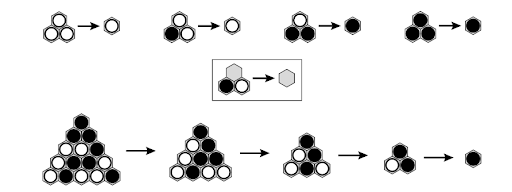
\includegraphics[width=0.6\linewidth]{Y-reduction.png}
                    \caption{Déroulement de BPR sur un jeu de Y. Figure de \cite{browne12}}
                    \label{fig:Y-reduction}
                \end{figure}
                \begin{figure}[H]
                    \centering
                    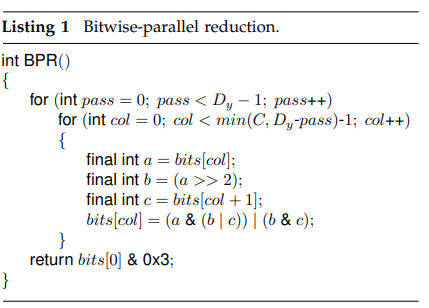
\includegraphics[width=0.5\linewidth]{BPR.png}
                    \caption{L'algorithme BPR. Figure de \cite{browne12}}
                    \label{fig:BPR}
                \end{figure}
            \end{enumerate}
        \end{itemize}
    \item Recherches de meilleurs coups et heuristiques :
        \begin{itemize}
            \item Heuristique pour minimax et alphabeta \textbf{F52} \ref{heuristique1} et \textbf{F58} \ref{heuristique2}
            \item Minimax \textbf{F53} \ref{minimax}
            \item $\alpha\beta$-pruning \textbf{F54} \ref{alphabeta}
            \item Monte-Carlo tree search \textbf{F56} \ref{MonteCarlo}
        \end{itemize}
\end{enumerate}

\section{Spécifications étendues des besoins}

Cette section regroupe l'ensemble des besoins du projet. Nous avons choisi de ne pas faire de liste précise contenant un ensemble de besoins à implémenter, mais nous les avons au lieu de cela triés par "versions", chaque version du projet étant associé à une semaine quant à sa sortie. La première version du projet implémentera des besoins fondamentaux, puis les suivantes des besoins jugés de moins en moins importants.

\subsection{Besoins transverses}

Cette section contient l'ensemble des besoins non fonctionnels, transverses au projet.

\medskip
\begin{itemize}
    \item \textbf{F1 :} Langage
    \begin{itemize}
        \item Le code source du programme sera en Python (3.7)
    \end{itemize}
    \item \textbf{F2 :} Style de codage
    \begin{itemize}
        \item Le code source respectera le style de codage PEP8
    \end{itemize}
    \item \textbf{F3 :} Langue
    \begin{itemize}
        \item La documentation, les variables, les fonctions, les fichiers, etc, seront en anglais
    \end{itemize}
    \item \textbf{F4 :} Système cible
    \begin{itemize}
        \item GNU/Linux
        \item Tester et développer sur Ubuntu 20.04 entre autres.
    \end{itemize}
    \item \textbf{F5 :} Documentation
    \begin{itemize}
        \item Un manuel utilisateur expliquant les fonctionnalités et les règles du jeu sera présent.
        \item Une option d’aide en ligne de commande (\textbf{F16}) sera présente pour assister l'utilisateur quand il veut lancer le programme.
        \item Des commentaires dans le code source aideront à la compréhension et la maintenabilité du programme.
    \end{itemize}
    \item \textbf{F6 :} Tests
    \begin{itemize}
        \item 80\% du code est couvert par les tests. Les tests doivent être automatisés et faciles à lancer.
    \end{itemize}
    \item \textbf{F7 :} Bugs
    \begin{itemize}
        \item "aucun crash", les erreurs doivent afficher des messages d’erreur.
    \end{itemize}
    \item \textbf{F8 :} Performances
    \begin{itemize}
        \item Un document présentera les performances (avec le matériel utilisé) des différents algorithmes complexes sur différentes entrées ainsi que les performances obtenues lors d'une exécution dans un contexte donné (Chargement de l'interface graphique, mise à jour de l'interface graphique, chargement et sauvegarde d'une partie).
    \end{itemize}
    \item \textbf{F9 :} Build system
    \begin{itemize}
        \item pyproject.toml + setuptools
        \item Nécessite de créer un fichier .toml. On y spécifiera au moins les auteurs, les dépendances, le nom, la version, la version de python et la description du projet.
    \end{itemize}
    \item \textbf{F10 :} Framework de tests
    \begin{itemize}
        \item pytest + coverage
        \item Exploitation du module pytest.mocking pour utiliser les mocks et spy pour vérifier les entrées, les sorties, les appels de fonction, etc.
    \end{itemize}
    \item \textbf{F11 :} Module de gestion des options en ligne de commande
    \begin{itemize}
        \item argparse
    \end{itemize}
    \item \textbf{F12 :} Bibliothèque graphique
    \begin{itemize}
        \item PyGObject
    \end{itemize}
\end{itemize}

\subsection{Version 1.0 - Semaine 1 : Exécutable de base}

\medskip
\begin{itemize}
    \item \textbf{F42 :} Plateau de jeu
    \begin{itemize}
        \item \textbf{Besoin fonctionnel}
        \item \textbf{Description :} Des bitboards représenteront l’état du plateau de jeu à chaque instant.
        \item \textbf{Prérequis :} Module bitboard (\textbf{F43}).
        \item \textbf{Actions :} Implémenter la classe Board qui a pour un attribut 2 bitboards, un pour chaque joueur qui représente l’état du plateau. En plus de getters, les méthodes à implémenter sont toutes celles qui manipulent les bitboards du plateau (reset, add\_move, check\_legal\_move, remove\_move). reset réinitialise les bitboards; add\_move ajoute un bit au bitboard correspondant au joueur courant; remove\_move; check\_legal\_move renvoie True si les bits des 2 bitboards sont à 0 et False sinon.
        \item \textbf{Tests :} Les tests de récupération de cette structure se trouvent dans le module game (\textbf{F44.1}).
    \end{itemize}
\bigskip
    \item \textbf{F44 :} État du jeu
    \begin{itemize}
        \item \textbf{Besoin fonctionnel}
        \item \textbf{Description :} L’état du jeu est représenté par une structure de donnée qui contiendra :
        \begin{itemize}
            \item le joueur courant
            \item le tour actuel
            \item les temps restants pour chaque joueur si la partie est en mode blitz
            \item l’état du plateau de jeu
            \item l'historique des tours joués
        \end{itemize}
        Cette structure est la structure principale manipulée lors du fonctionnement du jeu.
        \item \textbf{Actions :} Créer une structure de données représentant le joueur courant par un 0 ou un 1, la structure qui contient et manipule les temps des joueurs, la structure contenant l’état du plateau, la structure contenant l’historique des tours joués et la configuration qui représente les informations du fichier de configuration et les options passées en arguments du programme. On doit pouvoir récupérer les différents composants afin de les manipuler pour le fonctionnement du jeu.
        \item \textbf{F44.1 :} Module game \label{game_state}
        \begin{itemize}
            \item \textbf{Description :} Structure game et fonctions associées :
            \begin{itemize}
                \item joueur courant
                \item plateau de jeu - bitboards
                \item couple d’historiques
                \item structure configuration
            \end{itemize}
            \item \textbf{Prérequis :} Plateau de jeu (\textbf{F42}), module bitboard (\textbf{F43}).
            \item \textbf{Actions :} Constructeur + getters de chacun des attributs + setters configuration + méthodes pour passer au tour ou au joueur suivant ou précédent.
            \item \textbf{Tests :} Vérifier les valeurs de retour des getters, les valeurs des modifications des setters et l’état de la structure obtenue à partir du constructeur.
        \end{itemize}
    \end{itemize}
\bigskip
    \item \textbf{F43 :} Module bitboard \label{bitboard}
    \begin{itemize}
        \item \textbf{Besoin fonctionnel}
        \item \textbf{Prérequis :} Aucun.
        \item \textbf{Description :} Ce module rassemble les fonctions qui permettent de manipuler les bitboards pour ce jeu.
        \item \textbf{Actions :} Implémenter une structure de donnée représentant un bitboard en utilisant le module bitarray et en fournissant des méthodes permettant la réalisation des différentes manipulations utiles au jeu (vérifier s'il y a une ligne (\textbf{F37}), réinitialiser les bitboards si on recommence une partie (\textbf{F36}), vérifier si une case est vide (\textbf{F29.2}) et changer la valeur d'un bit (\textbf{F29.3})).
        \item \textbf{Tests :} Le module bitarray peut être testé avec bitarray.test(). Les tests des algorithmes spécifiques sont renseignés dans les besoins \textbf{F29} (coups légaux et jouer un coup),  \textbf{F37} (détecter la fin de partie), \textbf{F36.1} (Recommencer une partie), etc.
    \end{itemize}
\bigskip
    \item \textbf{F29 :} Notation des coups
    \begin{itemize}
        \item \textbf{Besoin fonctionnel}
        \item \textbf{Description :} Le programme devra permettre de déplacer les pions. et s’assurer que les règles sont suivies. Si un coup est illégal (comme placer un pion hors du plateau ou sur une case déjà occupée), un message d’erreur sera affiché et le programme demandera un autre coup à l’utilisateur. 
        \item \textbf{Sous-besoin(s) :}
        \begin{itemize}
            \smallskip
            \item \textbf{F29.1 :} Récupérer le coup de l’utilisateur
            \begin{itemize}
                \item \textbf{Description :} L’utilisateur peut écrire son coup à jouer dans la console sous la forme “e4”, “i9”.
                \item \textbf{Prérequis :} Obtenir les commandes de l'utilisateur (\textbf{F26.1}).
                \item \textbf{Actions :} La fonction read\_user\_input() (\textbf{F26.1}) lit le contenu de la console et récupère le coup. On traduit ensuite ce coup grâce à une fonction \textit{translate(String pos)} qui prend en entrée la position sous la forme lettre/chiffre et vérifie si c’est un coup à jouer. Si ce n’est pas un coup à jouer, afficher un message d'erreur “invalid move” et afficher l’aide (Vérifier par exemple dans une partie de taille 9x9 que la première lettre n’est pas ‘j’ la 10ème lettre de l’alphabet).
                \item \textbf{Tests :} Selon la taille NxN du jeu, vérifier la sortie standard toutes les entrées correctes et quelques entrées incorrectes aléatoires.  
            \end{itemize}
            \smallskip
            \item \textbf{F29.2 :} Vérifier si le coup est légal
            \begin{itemize}
                \item \textbf{Description :} Le programme doit savoir si un coup est légal ou non.
                \item \textbf{Prérequis :} Récupérer le coup de l'utilisateur (\textbf{F29.1}).
                \item \textbf{Actions :} Implémenter une fonction check\_legal\_move qui renvoie True si un coup est légal en utilisant le module défini par \textbf{F43} selon l’algorithme de \ref{bitalgo}. Cette fonction doit lever une exception si le coup est hors du plateau. Elle renvoie False et affiche "Space already occupied" quand la case est déjà occupée.
                \item \textbf{Tests :} Test général spécifié juste en dessous au besoin \textbf{F29.3}.
            \end{itemize}
            \smallskip
            \item \textbf{F29.3 :} Jouer un coup
            \begin{itemize}
                \item \textbf{Description :} Vérifier si la case est vide, jouer le coup si oui, afficher un message d’erreur sinon.
                \item \textbf{Prérequis :} Vérifier si le coup est légal et le jouer (\textbf{F29.2}), Module configuration (\textbf{F44.3}).
                \item \textbf{Actions :} Implémenter une fonction make\_move qui vérifie si le coup est légal, accède à l’état du jeu pour modifier le bitboard des pièces du joueur courant et le bitboard des cases libres si oui, affiche un message d’erreur et redemande un coup à jouer sinon.
                \item \textbf{Tests :} Sur un plateau de taille NxN vide, jouer sur chaque position puis, lorsqu'il sera plein, rejouer sur chaque position. Vérifier pendant la première moitié qu'il n'y ait pas d'erreur levée et que la valeur de retour est True. Vérifier lors de la seconde moitié qu'aucune erreur n'est levée et que le bon message s'affiche. Ensuite, sur un nouveau plateau, vérifier que des coups hors du plateau (>$N^2$) lèvent l'erreur. On pourra tester avec $N^2$ et un nombre aléatoire supérieur à $N^2$. Vérifier à chaque coup que l'état du bitboard ne change qu'à la position voulue en comparant bit par bit les bitarray.
            \end{itemize}
            \smallskip
            \item \textbf{F29.4 :} Afficher le coup joué sur le plateau
            \begin{itemize}
                \item \textbf{Description :} L’affichage du plateau est mis à jour avec le nouveau coup joué.
                \item \textbf{Prérequis :} Jouer un coup (\textbf{F29.3}), affichage du plateau (\textbf{F28}).
                \item \textbf{Actions :} Rien à faire si F28 est implémentée correctement.
                \item \textbf{Tests :} Lire la sortie standard et vérifier que le coup joué se trouve au bon endroit.
            \end{itemize}
        \end{itemize}
    \end{itemize}
\bigskip
    \item \textbf{F28.1 :} Affichage du plateau
    \begin{itemize}
        \item \textbf{Besoin fonctionnel}
        \item \textbf{Description :} Afficher l’état du plateau sur la sortie standard après chaque coup. Chaque joueur est représenté par des caractères différents, ’X’ pour les noirs et ’O’ pour les blancs et les cases vides par un ’.’.
        \item \textbf{Prérequis :} État du plateau (\textbf{F44}).
        \item \textbf{Actions :} Une fonction board\_to\_string traduire le plateau actuel en string afin de le print.
        \item \textbf{Test :} Vérifier la sortie écrite sur la sortie standard pour un plateau vide. (Plateau non vide testé dans l'affichage du coup joué sur le plateau (\textbf{F29.4})).
    \end{itemize}
\bigskip
    \item \textbf{F33.1 :} Quitter
    \begin{itemize}
        \item \textbf{Besoin fonctionnel}
        \item \textbf{Description :} L’utilisateur peut quitter la partie en entrant la commande ‘quit’ ou ‘q’.
        \item \textbf{Prérequis :} Obtenir les commandes de l’utilisateur (\textbf{F26.1}), obtenir l’accord du joueur (\textbf{F26.2}).
        \item \textbf{Actions :} Ajouter la détection des commandes ‘quit’ et ‘q’ à la fonction read\_user\_input. Elle appelle ensuite la fonction confirm pour demander à l’utilisateur s'il est sûr de quitter le programme. Si oui quitter le programme, continuer la partie sinon.
        \item \textbf{Tests :} Vérifier que le programme se termine et renvoie 0 si on entre ‘quit’ puis ‘y’ et vérifier que le programme continue en jouant quelques coups si on entre ‘q’ et ‘n’.
    \end{itemize}
\bigskip
    \item \textbf{F61 :} Gameloop CLI
    \begin{itemize}
        \item \textbf{Besoin fonctionnel}
        \item \textbf{Description :} Le jeu comporte une boucle principale qui demande les commandes à l’utilisateur, fait alterner les joueurs et s’occupe des transitions entre les tours.
        \begin{itemize}
        	\item Un tour du point de vue de l’utilisateur, ressemble à : (version ligne de commande) on affiche le plateau, les joueurs peuvent taper “-h”/”--help” pour afficher les commandes disponibles, le premier joueur à jouer est le blanc, on passe au tour du suivant lorsque joueur blanc à input un move c.-à-d. une commande telle que 4f, on affiche le plateau, puis c’est ensuite au tour de joueur noir, qui a aussi accès au même commande, une fois qu’il a input un move, on reboucle.
        	\item Avant chaque coup, on s’assure qu’il est légal, s’il ne l’est pas, on ne joue pas le coup et on affiche le message “coup invalide, veuillez jouer un coup légal, –help pour voir les règles du jeu”. 
        	\item Après chaque coup, on doit vérifier s'il y a un gagnant et si un gagnant il y a, alors on sort de la gameloop, on affiche le gagnant et on propose de refaire une partie. Si jeu lancé sur GUI on renvoie sur le menu principal.
        	\item Si jamais on souhaite changer les paramètres en ligne de commande, il faudra modifier le fichier config.chkrsrc, ou relancer le programme avec différentes options passées en ligne de commande.
            \item On doit aussi quitter la boucle de jeu si la commande quitter est pressée.
            Si restart est input réinitialiser les structures.
            Les deux joueurs ont aussi accès à annuler le tour précédent, cela doit donc se faire avant de jouer son coup, c.-à-d. si blanc joue alors, on enlève le coup précédent des deux joueurs et on affiche le plateau, c'est à blanc de jouer. Si noir le fait, alors on annule les deux derniers coups de blanc et le coup de noir. On affiche le plateau, c'est à noir de jouer. Moyennant une confirmation des deux joueurs
            Lors du premier tour, seulement le joueur noir à la possibilité d’utiliser swap, via la commande swap.
        \end{itemize}
        \item \textbf{Prérequis :} Obtenir les commandes de l’utilisateur (\textbf{F26.1}), aide en ligne de commandes (\textbf{F16}).
        \item \textbf{Actions :} Implémenter une fonction gameloop(), qui met en place la boucle de jeu, qui affiche le plateau,  récupère l’input du premier joueur (blanc) et le traite, si c’est un humain, on utilise la fonction \textit{read\_user\_input}, si c’est une IA, on utilise \textit{ai\_play\_move} définie dans le besoin \textbf{F25}. On refait la même chose pour le second joueur. On quitte cette fonction si jamais la commande quit ou restart est passée, ou si un joueur gagne.
        \item \textbf{Tests :} Cette fonction utilisera principalement les fonctions mises en place par les autres besoins et donc testés, on doit s’assurer que ces fonctions sont appelées au bon moment. Via un script, on peut lancer gameloop et entrer en ligne de commande quit, et vérifier que l’on quitte le programme, et que cela ne se déroule pas lors d’autre commande. Vérifier que swap soit seulement possible lors du premier tour par le joueur noir. Via un script, on doit pouvoir faire swap avec le joueur blanc et constater que le plateau reste identique et que l’on a un message indiquant l’impossibilité d’utiliser swap par le joueur blanc. Pareil pour le joueur noir lorsque le premier tour est passé.Vérifier  que la fonction ai\_play\_move joue un coup valide et de la bonne couleur, pour cela, on compare le plateau avant et après appel de la fonction, ils doivent avoir un coup d’écart, et de la couleur passée en paramètre.
    \end{itemize}
\bigskip
    \item \textbf{F26 :} Interface en ligne de commande
    \begin{itemize}
        \item \textbf{Besoin fonctionnel}
        \item \textbf{Sous-besoin(s) :}
        \begin{itemize}
            \smallskip
            \item \textbf{F26.1 :} Obtenir les commandes de l’utilisateur
            \begin{itemize}
                \item \textbf{Description :} Le programme devra posséder une interface en ligne de commande qui permette une interaction avec l’utilisateur via le terminal. Cette interface textuelle sera lancée par défaut par le programme. 
                \item \textbf{Description :} Le programme peut récupérer les commandes écrites par l’utilisateur.
                \item \textbf{Actions :} Implémenter une fonction read\_user\_input qui lit l’entrée standard et, selon l’entrée, appelle la fonction appropriée. Par défaut, envoyer un message d’erreur “wrong input” et afficher l’aide avant de redemander une entrée à l’utilisateur.
                \item \textbf{Tests :} Vérifier que la fonction affiche les bons messages avec une entrée incorrecte.
            \end{itemize}
            \smallskip
            \item \textbf{F26.2 :} Obtenir l’accord du joueur
            \begin{itemize}
                \item \textbf{Description :} Certaines interactions nécessitent une réponse par oui ou par non du joueur.
                \item \textbf{Actions :} une fonction booléenne confirm affiche un message passé en paramètre puis affiche la question “yes or no ? (y/n)”, lit l’entrée standard et renvoie True si elle lit ‘y’ ou ‘o’, False si elle lit ‘n’ ou envoie le message “respond by typing ‘y’ or ‘n’” sinon.
                \item \textbf{Tests :} Vérifier les messages en lisant la sortie standard et la valeur de retour de la fonction avec ‘y’, ‘o’, ‘n’ et une entrée quelconque.
            \end{itemize}
        \end{itemize}
    \end{itemize}
\bigskip
    \item \textbf{F37 :} Fin de partie
    \begin{itemize}
        \item \textbf{Besoin fonctionnel}
        \item \textbf{Description :} Le programme doit détecter la fin de la partie et afficher le résultat de la partie ainsi que le gagnant s’il y en a un.
        \item \textbf{Sous-besoin(s) :}
        \begin{itemize}
            \smallskip
            \item \textbf{F37.1} Détecter la fin de partie
            \begin{itemize}
                \item \textbf{Prérequis :} État du plateau (\textbf{F44}). 
                \item \textbf{Actions :} Requiert une fonction is\_game\_over(board) → (boolean, winner). Renvoie True si la partie est finie, False sinon. Si fin de partie il y a, la fonction renvoie aussi le joueur gagnant. Elle appelle la détection de connexion définie dans le module bitboard (\textbf{F43}).
                \item \textbf{Tests :} Vérifier que la fonction renvoie True et le joueur gagnant si on lui passe un plateau gagnant en paramètre et qu’elle renvoie False pour un plateau quelconque.
            \end{itemize}
            \smallskip
            \item \textbf{F37.2} Affichage de la fin de partie
            \begin{itemize}
                \item \textbf{Prérequis :} État du plateau, joueur courant (\textbf{F44}).
                \item \textbf{Actions :} Écrire le gagnant sur la sortie standard lorsque la partie est terminée.
                \item \textbf{Tests :} Lire la sortie standard et vérifier que le message soit correct.
            \end{itemize}
        \end{itemize}
    \end{itemize}
\bigskip
    \item \textbf{F13.1 :} Créer un fichier de langages pour le module de framework d’internationalisation gettext
    \begin{itemize}
        \item \textbf{Besoin fonctionnel}
        \item \textbf{Action :} créer un fichier pouvant être utilisé par le module gettext. Ce fichier contiendra l’ensemble des strings du jeu (utilisateur), identifiés par un id, avec, pour chacun, leurs différentes traductions dans les langages voulus. Dans le code, on devra spécifier le langage afin que le module gettext puisse automatiquement afficher le bon string en fonction de son id et du langage.
    \end{itemize}
\end{itemize}

\subsection{Version 1.5 - Semaine 2 : Sauvegarde et chargement}

\medskip
\begin{itemize}
    \item \textbf{F44.2 :} Historique des coups joués
    \begin{itemize}
        \item \textbf{Description :} Couple d’historiques et fonctions associées :
        \begin{itemize}
            \item Pile de coup joués
            \item Pile de coup annulés 
        \end{itemize}
        \item \textbf{Prérequis :} Module de l'historique des coups joués (\textbf{F30.2}).
        \item \textbf{Actions :} getters de chacun des historiques.
        \item \textbf{Tests :} Vérifier la valeur de retour des getters.
    \end{itemize}
\bigskip
    \item \textbf{F40 :} Format de l’historique
    \begin{itemize}
        \item \textbf{Besoin Fonctionnel}
        \item \textbf{Description :} On doit être capable de récupérer des historiques à partir de fichier .hexhistory. Les fichiers de type .hexhistory, contiennent une section commentaire optionnel, et une section historique obligatoire, chaque section est comprise entre deux symboles ‘\#’. La section historique : chaque ligne contient un tour, chaque ligne est séparée par un symbole ‘\$’. Un tour se compose de deux coups, celui de joueur blanc puis celui du joueur noir, un coup se compose d’un caractere et d’un int (colonne, ligne). 
        \item \textbf{Prérequis :} Module de l'historique des coups (\textbf{F30.2}).
        \item \textbf{Actions :}
        \begin{itemize}
            \item load\_history\_from\_file(file\_t file)
            \item save\_history\_to\_history\_file(File output\_file) (On ne sauvegarde que l’historique des coups joués.)
        \end{itemize}
        \item \textbf{Tests :} save\_history\_to\_history\_file doit créer ou remplir un fichier en suivant le format, donc lors de l’utilisation de save\_history\_to\_history\_file sur un fichier sauvegardé, on ne doit pas avoir d’erreur. Vérifier que load\_history\_from\_file renvoie une erreur sur un fichier ne suivant pas exactement le format. 
    \end{itemize}
\bigskip
    \item \textbf{F33 :} Quitter et sauvegarder une partie
    \begin{itemize}
        \item \textbf{Description :} Le programme devra permettre de quitter une partie en cours et de la sauvegarder dans un fichier. 
        \item \textbf{Sous-besoin(s) :}
        \begin{itemize}
            \smallskip
            \item \textbf{F33.1 :} Quitter
            \begin{itemize}
                \item \textbf{Description :} L’utilisateur peut quitter la partie en entrant la commande ‘quit’ ou ‘q’.
                \item \textbf{Prérequis :} Obtenir les commandes de l’utilisateur (\textbf{F26.1}), obtenir l’accord du joueur (\textbf{F26.2}).
                \item \textbf{Actions :} Ajouter la détection des commandes ‘quit’ et ‘q’ à la fonction read\_user\_input. Elle appelle ensuite la fonction\textit{ confirm} pour demander à l’utilisateur s'il est sûr de quitter le programme. Si oui quitter le programme, continuer la partie sinon.
                \item \textbf{Tests :} Vérifier que le programme se termine et renvoie 0 si on entre ‘quit’ puis ‘y’ et vérifier que le programme continue en jouant quelques coups si on entre ‘q’ et ‘n’.
            \end{itemize}
            \smallskip
            \item \textbf{F33.2 :} Sauvegarder
            \begin{itemize}
                \item \textbf{Description :} L’utilisateur peut demander de sauvegarder une partie en cours.
                \item \textbf{Prérequis :} Obtenir les commandes de l’utilisateur (\textbf{F26.1}), format de fichier (\textbf{F39}).
                \item \textbf{Actions :} Ajouter la détection des commandes ‘save’ et ‘s’ à la fonction read\_user\_input. Les spécificités sont renseignées dans F39.
                \item \textbf{Tests :} Vérifier que les commandes ‘save’ et ‘s’ avec et sans chemin créent le bon fichier au bon endroit.
            \end{itemize}
            \smallskip
            \item \textbf{F33.3 :} Quitter et sauvegarder
            \begin{itemize}
                \item \textbf{Description :} Lorsque l’utilisateur souhaite quitter la partie, le jeu lui demande s'il veut sauvegarder.
                \item \textbf{Prérequis :} quitter (\textbf{F33.1}), sauvegarder (\textbf{F33.2}), obtenir les commandes de l’utilisateur (\textbf{F26.1}), format de fichier (\textbf{F39}).
                \item \textbf{Actions :} Rajouter un appel à confirm pour demander si l’utilisateur veut quitter et sauvegarder. Si oui, avant de quitter, demander le chemin relatif, sauvegarder à l’emplacement spécifié et quitter, quitter sinon.
                \item \textbf{Tests :} Vérifier que, dans les 2 cas, avec ‘quit’, le programme renvoie 0 et vérifier que le fichier est correct avec ‘quit’, ‘y’ puis <path>.
            \end{itemize}
        \end{itemize}
    \end{itemize}
\bigskip
    \item \textbf{F30 :} Représentation de l’historique
    \begin{itemize}
        \item \textbf{Besoin Fonctionnel}
        \item \textbf{Description :} L’historique sera représenté comme une liste des tours du jeu. Par exemple, le premier tour sera affiché comme suit : "1. O h4 X e3" (le numéro du tour dans la partie, le joueur puis la case où est placé le nouveau pion). Les accolades ’{}’ signalent un commentaire qui sera ignoré par le parseur.
        \item \textbf{Sous-besoin(s) :}
        \begin{itemize}
            \smallskip
            \item \textbf{F30.1 :} Stocker les coups joués à chaque tour
            \begin{itemize}
                \item \textbf{Description :} Dès que le deuxième joueur finit son tour, on doit pouvoir récupérer les coups joués lors de ce tour.
                \item \textbf{Actions :}  À chaque tour, sauvegarder les coups joués dans une variable puis, à la fin du tour, les ajouter à l’historique des coups joués.
                \item \textbf{Tests :} Vérifier la valeur de la tête de pile de l’historique des coups joués lorsqu’un tour se finit.
                \item \textbf{Prérequis :} Module pour l'historique des coups (\textbf{F30.2}).
            \end{itemize}
            \smallskip
            \item \textbf{F30.2 :} Module pour l'historique des coups
            \begin{itemize}
                \item \textbf{Description :} Le module rassemble les fonctions qui permettent de manipuler l’historique des coups joués.
                \item \textbf{Actions :} Implémenter une structure de données représentant l’historique en utilisant 2 piles manipulant des triplets (nb\_tour, joueur, coup). Les piles sont représentées à l’aide du module collection.deque qui offre des opérations append et pop en temps constant. La première représente les coups joués et la deuxième les coups annulés. Si un coup est joué alors que des coups ont été annulés, vider la deuxième pile. Le mécanisme de LIFO des piles se prête bien à la représentation d’un historique.
                \item \textbf{Tests :} Vérifier le bon comportement de chaque fonction. append, pop, is\_empty.
                \item \textbf{Prérequis :} Récupérer le coup de l’utilisateur (\textbf{F29.1}).
            \end{itemize}
            \smallskip
            \item \textbf{F30.3 :} Affichage de l’historique
            \begin{itemize}
                \item \textbf{Description :} Sur l’interface en lignes de commande, afficher les 3 derniers tours et, si un coup est annulé, afficher le dernier coup annulé.
                \item \textbf{Prérequis :} Module pour l'historique des coups (\textbf{F30.2}).
                \item \textbf{Actions :} Parcourir l’historique des coups joués et afficher les 3 premiers tours et afficher, si elle n’est pas vide, le tour en tête de l’historique des coups annulés.
                \item \textbf{Tests :} Vérifier la sortie standard après avoir joué quelques tours.
            \end{itemize}
        \end{itemize}
    \end{itemize}
\bigskip
    \item \textbf{F39 :} Format de fichier
    \begin{itemize}
        \item \textbf{Besoin Fonctionnel}
        \item \textbf{Prérequis :} Structures internes (\textbf{F42, F43, F44}).
        \item \textbf{Description :}  On décrit ici l'interaction de l'utilisateur avec les fichiers de sauvegarde, à l’aide de la commande save <path>/<nom(sans l’extension)>. Si path non spécifié, alors, on sauvegarde dans le répertoire où se situe l'exécutable. Si le nom est non spécifié alors le nom sera hexgame-<date + heure+minute+seconde> Si nom déjà pris alors, on rajoute 1, si déjà pris, on incrémente l’indice jusqu'à que l’on puisse sauvegarder. On doit aussi pouvoir écraser un fichier existant au même nom, pour cela, on utilise la fonction confirm puis on remplace le fichier existant si réponse oui. Pour charger une partie, l'utilisateur doit spécifier un chemin relatif, partant de l'exécutable jusqu’au fichier .hexgame. exemple load <path>. Load doit être capable de traiter les .hexgame et les .hexhistory. Pour changer une configuration, l'utilisateur doit modifier par lui-même le fichier configuration à la racine du programme. Ce qui implique que l’on doive créer un fichier .checkersrc s'il n’y en a pas à la racine. 3 types de fichiers différent historique(.hexhistory(\textbf{F40}), .hexgame, .checkersrc (\textbf{F41})) :
        \begin{itemize}
            \item .hexhisory contient uniquement un historique de coup, détaillé dans (\textbf{F40}).
            \item .checkersrc contient la configuration du jeu, détaillé dans (\textbf{F41}).
            \item .hexgame décrit le fichier sauvegardant une partie, il contient obligatoirement un plateau valide. Case vide symbolisée par ‘.’, pièce blanche  symbolisée ‘O’ et pièce noire symbolisée ‘X’. Il peut aussi contenir en entête un commentaire contenu entre les deux premières occurrences du symbole “\#”. S'ensuit le plateau, contenu entre 2e ‘\#‘ et 3e ‘\#’. Après le 2e \#, chaque ligne décrit une ligne du plateau. Chacune de ces lignes doit contenir au moins le nombre de symboles renseignés dans la configuration courante du jeu, si ce n’est pas le cas, alors on renvoie une erreur (raise TypeError("Missing character in game file")). Entre 3e’\#’ et 4e’\#’ historique de coups, chaque ligne décrit un tour, entre chaque ligne il y’a un séparateur ‘\$’. Une ligne décrie d’abord le coup du joueur blanc puis celui du joueur noir. Un coup se compose de 2 caractères, une lettre décrivant la colonne et un entier. Si la ligne ne suit pas exactement ce format alors, on renvoie une erreur (raise TypeError("Wrong move format line \%d",line)). entre 4e’\#’ et 5e’\#’ : joueur courant ‘X’ | ‘O’, actions load\_current\_player(File inputFile) et save\_current\_player(File outputFile, game\_t game).
            Le caractère ‘§’ symbolise une section optionnelle vide (Commentaire, historique).
        \end{itemize}
        \begin{figure}[H]
            \centering
            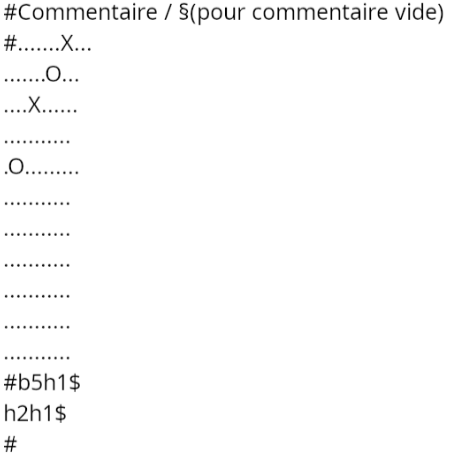
\includegraphics[width=0.50\linewidth]{images/hex_file_example.png}
            \caption{Exemple de fichier(.hexgame) pour un jeu de size 11 (on rajoute ‘\#’ à la fin) :}
        \end{figure}
        \item \textbf{Sous-besoin(s) :} 
        \begin{itemize}
            \smallskip
            \item \textbf{F39.1 :} Lire fichier de jeu (.hexgame)
            \begin{itemize}
                \item \textbf{Actions :} Implémenter les fonctions \textit{String get\_comment(file\_t file)}, \textit{history get\_history\_from\_file(file)}
                \item \textbf{Tests :} Sauvegarder une partie dans un fichier, puis charger cette dernière dans de nouvelles structures internes, on compare alors les structures, elles doivent être identiques.
            \end{itemize}
            \smallskip
            \item \textbf{F39.2 :} Sauvegarder partie dans un fichier (.hexgame)
            \begin{itemize}
                \item \textbf{Actions :} Implémenter les fonctions \textit{save\_game\_as\_file(game, file output)}, \textit{save\_game\_as\_file\_without\_history(game, file)} et \textit{add\_comment(String input)}
                \item \textbf{Tests :} Sauvegarder le jeu puis le load vérifier que les deux structures internes sont identiques, vérifier que si on utilise \textit{save\_game\_as\_file\_without\_history}; on récupère un historique vide, concernant le format si jamais la fonction load renvoie une erreur alors le test renvoie faux.
            \end{itemize}
            \smallskip
            \item \textbf{F39.3 :} Remplacer structures internes, par l’état de jeu spécifié dans un fichier (.hexgame)
            \begin{itemize}
                \item \textbf{Actions :} Implémenter les fonctions \textit{load\_game\_from\_file(file)} (renvoie une erreur si incapable de récupérer une section/ fichier ne correspond pas au format décrit) et \textit{load\_history\_from\_file(file)}
                \item \textbf{Tests :} On sauvegarde puis on charge, dans une structure game, on doit avoir les deux structures identiques et vérifier que l’on  renvoie une erreur si le fichier donné ne correspond pas au bon format.
            \end{itemize}
        \end{itemize}
    \end{itemize}
\bigskip
    \item \textbf{F32 :} Affichage des messages
    \begin{itemize}
        \item \textbf{Besoin Fonctionnel}
        \item \textbf{Description :} Le programme devra afficher des messages d’information pendant la partie en fonction du mode dans lequel il est (default, verbose, debug).
        \item \textbf{Prérequis :} Interface en ligne de commande (\textbf{F26})
        \item \textbf{Actions :} Si le jeu est en mode verbose et/ou en mode debug, une fonction de signature \textit{info(mode, message)}, appelée lorsque cela est pertinent dans chaque partie du programme, affiche le message “message” si le jeu est en mode “mode”.
        \item \textbf{Tests :} Vérifier que la fonction info marche sans mode et avec les modes verbose et debug.
    \end{itemize}
\bigskip
    \item \textbf{F15 :} Syntaxe de lancement du programme : hex [OPTIONS] [FILENAME]
    \begin{itemize}
        \item \textbf{Besoin Fonctionnel}
        \item \textbf{Description :} Le programme doit être lancé via une syntaxe précise et donner la possibilité de spécifier des options ainsi qu'un fichier en entrée.
        \item \textbf{Sous-besoin(s) :}
        \begin{itemize}
            \smallskip
            \item \textbf{F15.1 :} Vérification des options spécifiées en ligne de commande
            \begin{itemize}
                \item \textbf{Actions :} Analyser les paramètres du programme avec un parseur à construire créé avec le module argparse. Afficher un message d’erreur et une aide en cas d’option invalide. Doit suivre l’implémentation des différentes options en ligne de commande (\textbf{F16 à F25}). Les paramètres récupérés doivent écraser les valeurs obtenues à partir de la lecture du fichier de configuration.
                \item \textbf{Tests :} Le module argparse pourra être testé sur différents paramètres du programme afin de vérifier que les paramètres valides ou non soient correctement parsés/évalués.
            \end{itemize}
            \smallskip
            \item \textbf{F15.2 :} Vérification des fichiers spécifiés en ligne de commande
            \begin{itemize}
                \item \textbf{Prérequis :} Obtenir les commandes de l’utilisateur (\textbf{F26.1}), Affichage de la fin de partie (\textbf{F37.2})
                \item \textbf{Actions :} Analyser les paramètres du programme avec le module argparse. Afficher un message d’erreur et une aide en cas de fichier invalide. Vérifier aussi les extensions des fichiers.
                \item \textbf{Tests :} Tester sur des fichiers valides et invalides avec des extensions valides et invalides.
            \end{itemize}
            \smallskip
            \item \textbf{F15.3 :} Code de retour de programme
            \begin{itemize}
                \item \textbf{Actions :} Renvoyer 1 en cas d’erreur sinon 0 en fin de programme.
                \item \textbf{Tests :} Exécuter le programme sur des entrées de sorte qu'il se termine en renvoyant un code d’erreur spécifique qu’il faudra vérifier (exemple : lancer avec ’-V’ et vérifier que le programme se termine avec un code 0).
            \end{itemize}
        \end{itemize}
    \end{itemize}
\bigskip
    \item \textbf{F31 :} Abandon
    \begin{itemize}
        \item \textbf{Besoin Fonctionnel}
        \item \textbf{Description :} Le joueur courant peut abandonner la partie en cours en entrant “abandon” ou “give up” ou “gu” dans la console.
        \item \textbf{Prérequis :} Obtenir les commandes de l’utilisateur (\textbf{F26.1}), Affichage de la fin de partie (\textbf{F37.2})
        \item \textbf{Actions :} Modifier la fonction \textit{read\_user\_input} pour lire et prendre en compte les entrées décrites dans la description. L’abandon déclenche l’affichage des résultats et l’arrêt de la partie définis dans \textbf{F37.2}.
        \item \textbf{Tests :} Les commandes “abandon”, “give up” et “gu” doivent être reconnues, elles ne doivent pas renvoyer d’erreur directement. On charge une partie en cours puis on teste ces trois commandes. L’état du jeu doit passer à “terminé” (on ne peut plus jouer de coups ni “undo” un coup etc) et le joueur qui abandonne doit être déclaré perdant.
    \end{itemize}
\bigskip
    \item \textbf{F16 :} Aide en ligne de commandes
    \begin{itemize}
        \item \textbf{Besoin Fonctionnel}
        \item \textbf{Description :} Possibilité d’afficher l’aide du programme puis quitter via une option en ligne de commande.
        \item \textbf{Prérequis :} Vérification des options en ligne de commande (\textbf{F15.1}).
        \item \textbf{Actions :} À l’aide du module argparse (\textbf{F11}), on doit pouvoir reconnaître l’option “-h”/”--help” puis afficher une description du programme et les différentes options disponibles sur la sortie standard (\textbf{F17, F18, F19, F20}), avant de terminer le programme en renvoyant 0.
        \item \textbf{Tests :} Vérifier que le programme affiche bien l’aide et renvoie 0 si lancé avec cette option.
    \end{itemize}
\bigskip
    \item \textbf{F17 :} Version
    \begin{itemize}
        \item \textbf{Besoin Fonctionnel}
        \item \textbf{Description :} Possibilité d’afficher la version du programme puis quitter via une option en ligne de commande.
        \item \textbf{Prérequis :} Vérification des options en ligne de commande (\textbf{F15.1}).
        \item \textbf{Actions :} À l’aide du module argparse (\textbf{F11}), on doit pouvoir reconnaître l’option “-V”/”--version” puis afficher la version courante du logiciel sur la sortie standard, avant de terminer le programme en renvoyant 0.
        \item \textbf{Tests :} Vérifier que le programme affiche sa version et renvoie 0 si lancé avec cette option.
    \end{itemize}
\bigskip    
    \item \textbf{F18 :} Mode verbose
    \begin{itemize}
        \item \textbf{Besoin Fonctionnel}
        \item \textbf{Description :} Possibilité d’afficher des informations supplémentaires durant l'exécution du jeu via une option en ligne de commande.
        \item \textbf{Prérequis :} Vérification des options en ligne de commande (\textbf{F15.1}).
        \item \textbf{Actions :} À l’aide du module argparse (\textbf{F11}), on doit pouvoir reconnaître l’option “-v”/”--verbose” et être capable de s’en souvenir pour afficher des informations supplémentaires durant l'exécution du jeu sur la sortie standard. Ajouter des print conditionnel qui affichent des informations pertinentes.
        \item \textbf{Tests :} Vérifier que le programme affiche bien les informations voulues dans la sortie standard si lancé avec cette option.
    \end{itemize}
\bigskip    
    \item \textbf{F19 :} Mode debug
    \begin{itemize}
        \item \textbf{Besoin Fonctionnel}
        \item \textbf{Description :} Possibilité d’afficher des informations de débogage durant l'exécution du jeu via une option en ligne de commande.
        \item \textbf{Prérequis :} Vérification des options en ligne de commande (\textbf{F15.1}).
        \item \textbf{Actions :} À l’aide du module argparse (\textbf{F11}), on doit pouvoir reconnaître l’option “-d”/”--debug” et être capable de s’en souvenir pour afficher des informations de débogage durant l'exécution du jeu (tel que le temps d'exécution) sur la sortie standard (variable booléenne ou fonction). Ajouter des print conditionnel qui affichent des informations pertinentes.
        \item \textbf{Tests :} Vérifier que le programme affiche bien les informations voulues dans la sortie standard si lancé avec cette option.
    \end{itemize}
\bigskip    
    \item \textbf{F23 :} Taille du plateau
    \begin{itemize}
        \item \textbf{Besoin Fonctionnel}
        \item \textbf{Description :} Permettre de spécifier la taille du plateau via une option en ligne de commande.
        \item \textbf{Prérequis :} Vérification des options en ligne de commande (\textbf{F15.1}).
        \item \textbf{Actions :} À l’aide du module argparse (\textbf{F11}), on doit pouvoir reconnaître l’option “-z SIZE”/”--size SIZE”. La taille SIZE est comprise entre 1 et 20, et est de 11 par défaut si l’option n’est pas spécifiée. Il faut convertir SIZE en int et vérifier que sa valeur est bien comprise dans l’intervalle demandé.
        \item \textbf{Tests :} Vérifier que la taille du plateau est correcte ou qu’une erreur est bien renvoyée en fonction de la taille spécifiée en ligne de commande.
    \end{itemize}
\bigskip
    \item \textbf{F13 :} Module de framework d’internationalisation gettext
    \begin{itemize}
        \item \textbf{F13.2 :} Spécifier le langage via une option en ligne de commande
        \begin{itemize}
            \item \textbf{Besoin Fonctionnel}
            \item \textbf{Description :} Laisser la possibilité à celui qui lance le jeu de spécifier un langage en ligne de commande.
            \item \textbf{Prérequis :} Vérification des options en ligne de commande (\textbf{F15.1}).
            \item \textbf{Actions :} Créer une option (“-l LANGAGE”, ”--langage LANGAGE”) que le module argparse (\textbf{F11}) doit pouvoir reconnaître et utiliser pour déterminer le langage.
            \item \textbf{Tests :} Vérifier que le module argparse (F11) reconnaisse correctement les différentes options de langages. Par exemple, si le programme est lancé avec l’option “-l ENG”, la variable servant à spécifier le langage du jeu devra bien signifier qu’il est en anglais.
        \end{itemize}
    \end{itemize}
\end{itemize}

\subsection{Version 2.0 - Semaine 3 : Config + Historique}

\medskip
\begin{itemize}
    \item \textbf{F38 :} Rejouer une partie
    \begin{itemize}
        \item \textbf{Besoin Fonctionnel}
        \item \textbf{Prérequis :} Structures internes (\textbf{F42}, \textbf{F44.2}), format d’historique (\textbf{F40}).
        \item \textbf{Sous-besoin(s) :}
        \begin{itemize}
            \smallskip
            \item \textbf{F38.1 :} Charger un état de jeu à partir d’un historique de coups
            \begin{itemize}
                \item \textbf{Actions :} Modifier les structures internes pour être en adéquation avec le jeu à la fin de l’historique de coups avec un fichier historique comme spécifié et une fonction de signature load\_from\_history(history).
                \item \textbf{Tests :}  À partir d’un plateau, créer un fichier historique, puis charger ce plateau et comparer si les deux plateaux sont alors identiques.  
            \end{itemize}
            \smallskip
            \item \textbf{F38.2 :} Naviguer au sein d’un historique de coups
            \begin{itemize}
                \item \textbf{Description :} L’interface en ligne de commande affiche l’historique de coup. L’utilisateur peut alors naviguer en entrant ‘n’ pour passer au coup suivant, et ‘p’ pour passer au coup précédent.
                \item \textbf{Prérequis :} Obtenir l’accord des deux joueurs (\textbf{F35.3}).
                \item \textbf{Actions :} Une replay\_mode\_user\_input similaire à read\_user\_input lit les commandes ‘n’, ‘next’, ‘p’, ‘precedent’ et ‘h’. ‘n’ et ‘next’ correspondent à redo, ‘p’ et ‘precedent’ correspondent à ‘undo’ et ‘h’ affiche une aide comportant les informations de ce mode spécifiquement.
                Tests : Vérifier le bon comportement des commandes en testant l’affichage pour ‘h’ et l’état des historiques pour le reste.
            \end{itemize}
            \smallskip
            \item \textbf{F38.3 :} Recommencer une partie depuis la position choisie
            \begin{itemize}
                \item \textbf{Description :} Lors de la navigation dans un historique de coup, l’utilisateur peut entrer ‘start’, pour recommencer une partie à partir de ce coup moyennant une confirmation.
                \item \textbf{Prérequis :} Gameloop, main, etc. (\textbf{F61}).
                \item \textbf{Actions :} Ajouter ‘start’ aux commandes de replay\_mode\_user\_input. Utiliser \textit{confirm} pour l’accord du joueur. Si oui, cela rebascule le jeu sur la boucle principale et vide l’historique des coups annulés, on continue le mode replay sinon.
                \item \textbf{Tests :} Créer un historique de coup à partir d’une partie. Charger la partie à partir de l’avant-dernier coup, annuler le dernier coup sur le plateau d’origine, les plateaux doivent alors être identiques.
            \end{itemize}
        \end{itemize}
    \end{itemize}
\bigskip
    \item \textbf{F35 :} Naviguer dans l’historique
    \begin{itemize}
        \item \textbf{Besoin Fonctionnel}
        \item \textbf{Description :} Il doit être possible de revenir en arrière ou d’aller en avant dans l’historique des coups joués si tous les joueurs humains sont d’accord.
        \item \textbf{Prérequis :} Représentation de l’historique {F30}.
        \item \textbf{Sous-besoin(s) :}
        \begin{itemize}
            \smallskip
            \item \textbf{F35.1 :} Récupérer la commande de navigation
            \begin{itemize}
                \item \textbf{Actions :} Ajouter la détection des commandes ‘undo’ et ‘redo’ à la fonction read\_user\_input.
                Tests : Vérifier que ces commandes sont reconnues et n’affichent pas une erreur.
                \item \textbf{Prérequis :} Obtenir les commandes de l’utilisateur (\textbf{F26.1}).
            \end{itemize}
            \smallskip
            \item \textbf{F35.2 :} Revenir en arrière et aller en avant
            \begin{itemize}
                \item \textbf{Actions :} Utiliser undo revient en arrière d’un coup en jouant un coup vide sur la case du tour. De plus, cela rajoute ce coup dans l’historique des coups annulés. Jouer un coup alors que des coups ont été annulés vide l’historique des coups annulés. Utiliser redo rejoue un coup annulé.
                \item \textbf{Tests :} Vérifier que l’utilisation de ‘undo’ et ‘redo’ manipule correctement les historiques et le nombre de coups en vérifiant leurs états.
                Prérequis : Module pour l'historique des coups (\textbf{F30.2}), jouer un coup (\textbf{F29.3}).
            \end{itemize}
        \end{itemize}
    \end{itemize}
\bigskip
    \item \textbf{F41 :} Fichier de configuration
    \begin{itemize}
        \item \textbf{Besoin Fonctionnel}
        \item \textbf{Description :} Le programme devra être capable de lire un fichier de configuration (.checkersrc) qui contiendra les options par défaut du programme. Ce fichier sera lu au démarrage du programme et les options qu’il contient seront utilisées par défaut. Pour chaque option, sa valeur sera délimitée par ”=” ex : (ai = None). Chaque option sera délimitée par un retour à la ligne. Si le fichier n'existe pas, on doit le créer avec des valeurs par défaut.
        \item \textbf{Prérequis :} Aucun.
        \item \textbf{Actions :} Requiert une fonction qui lit le fichier config.checkersrc le parcourt grâce au délimiteur ci-dessous, récupère la valeur de chaque option et modifie l'objet Config stocké dans l'état du jeu. Si le fichier n'existe pas, une autre fonction.
        \item \textbf{Tests :} On lit un fichier de configuration connu puis l’algorithme de test vérifie si toutes les options ont les bonnes valeurs.
    \end{itemize}
\bigskip
    \item \textbf{F44.3 :} Configuration
    \begin{itemize}
        \item \textbf{Description :} L'état du jeu stocke la configuration de la partie. La taille du plateau, mode blitz, mode ia, mode verbose, mode debug, ia\_players (X,O,A), le temps de base du blitz, heuristique utilisée, algorithme d'exploration choisie, profondeur d'exploration, temps de réflexion, swap et mode contest sont les variables dont les valeurs sont stockées dans la configuration. 
        \item \textbf{Actions :} Implémenter la classe Config qui a comme attribut un dictionnaire contenant toutes les options du jeu et qui a comme méthodes des getters et des setters.
        \item \textbf{Tests :} Vérifier la valeur de retour des getters et l’état de la structure obtenue à partir du constructeur et des setters.
    \end{itemize}
\end{itemize}

\subsection{Version 3.0 - Semaine 4 : Mode Blitz}

\medskip
\begin{itemize}
    \item \textbf{F20 :} Mode Blitz
    \begin{itemize}
        \item \textbf{Besoin fonctionnel}
        \item \textbf{Description :} possibilité de donner un temps limité aux joueurs via une option en ligne de commande. Si le temps d’un des joueurs est écoulé, il perd la partie automatiquement. L’affichage est défini dans l'affichage du temps restant (\textbf{F28.2}).
        \item \textbf{Sous-besoin(s) :}
        \begin{itemize}
            \smallskip
            \item \textbf{F20.1 :} Option en ligne de commande
            \begin{itemize}
                \item \textbf{Description :} ajout d’une option en ligne de commande afin de spécifier que le jeu de lance en mode blitz.
                \item \textbf{Actions :} À l’aide du module argparse (\textbf{F11}), on doit pouvoir reconnaître l’option “-b”/”--blitz”.
                Prérequis : vérification des options en ligne de commande (\textbf{F15-1}).
                \item \textbf{Tests :} vérifier que le programme soit bien en mode blitz si lancé avec cette option.
            \end{itemize}
            \smallskip
            \item \textbf{F20.2 :} Module blitztimer
            \begin{itemize}
                \item \textbf{Description :} Un module blitztimer gère et stocke le temps restant de chaque joueur.
                \item \textbf{Actions :} Une classe blitztimer possède deux entiers représentant respectivement le temps restant du premier joueur et le temps restant du deuxième joueur. Ces deux attributs sont par défaut à 180 000 (30min en centièmes de seconde spécifiée dans le fichier de configuration (\textbf{F41})). Un thread tourne pour mettre à jour l’un des deux attributs toutes les 0.01s (Voir threading.timer pour encapsuler la classe et la personnaliser). Il peut être arrêté ou peut être mis en pause selon un flag GAME\_PLAYING, GAME\_PAUSE ou GAME\_STOPPED par exemple. La durée de base peut être spécifiée (\textbf{F21}). Un thread évite d’utiliser sleep et de ralentir le programme.
                \item \textbf{Prérequis :} Fichier de configuration (\textbf{F41}) pour la durée par défaut si temps non spécifié (\textbf{F21}).
                \item \textbf{Tests :} il faudra tester les fonctions et variables de ce module sur une exécution du programme afin de vérifier que le temps s’écoule comme souhaité.
            \end{itemize}
            \smallskip
            \item \textbf{F20.3 :} Temps écoulé
            \begin{itemize}
                \item \textbf{Description :} en mode blitz, si le temps d’un joueur est écoulé, il perd automatiquement.
                \item \textbf{Actions :} le module blitztimer (\textbf{20.2}) doit évaluer si un joueur atteint son temps max chaque fois que le timer est mis à jour (via une boucle if), auquel cas la partie doit se finir est le joueur n’ayant plus de temps est perdant.
                \item \textbf{Prérequis :} Module blitztimer (\textbf{20.2}), fin de partie (\textbf{F37.1}).
                \item \textbf{Tests :} le jeu pourra être lancé avec un temps extrêmement faible afin de vérifier que la partie se termine automatiquement avec le premier joueur perdant.
            \end{itemize}
        \end{itemize}
    \end{itemize}
\bigskip
    \item \textbf{F22 :} Changement de couleur / Inversion  des joueurs
    \begin{itemize}
        \item \textbf{Besoin fonctionnel}
        \item \textbf{Description :} permettre au second joueur de prendre la place du premier (uniquement après qu’il a joué son premier coup) s’il le souhaite via une option en ligne de commande ou via l’interface graphique (le premier joueur a un avantage considérable dans le jeu de hex. La règle de swap oblige le premier joueur à jouer de manière plus équitable au premier tour).
        \item \textbf{Sous-besoins :}
        \begin{itemize}
            \smallskip
            \item \textbf{F22.1 :} Option en ligne de commande
            \begin{itemize}
                \item \textbf{Description :} ajout d’une option en ligne de commande afin de spécifier que le jeu se lance avec cette option.
                \item \textbf{Prérequis :} vérification des options en ligne de commande (\textbf{F15.1}).
                \item \textbf{Actions :} À l’aide du module argparse (\textbf{F11}), on doit pouvoir reconnaître l’option “-s”/”--swap”.
                \item \textbf{Test :} vérifier que le programme soit bien dans ce mode si lancé avec cette option.
            \end{itemize}
            \smallskip
            \item \textbf{F22.2 :} Choix d’échange de couleur
            \begin{itemize}
                \item \textbf{Description :} si le jeu est lancé dans ce mode, il faut pouvoir proposer au second joueur d’inverser avec le premier.
                \item \textbf{Prérequis :} interface en ligne de commande (\textbf{F26.2}) ou interface graphique (\textbf{F27}).
                \item \textbf{Actions :} Si affiché dans le terminal, le programme devra demander un input au second joueur “do you wish to take the first player’s place ? (y/n)”. Si lancé avec une interface graphique, il faudra faire une fenêtre spécifique avec deux boutons pour poser la même question.
                \item \textbf{Tests :}  lire la sortie standard après le premier coup pour vérifier que le joueur ait le choix d’inverser sa couleur avec le premier.
            \end{itemize}
            \smallskip
            \item \textbf{F22.3 :} Échange de couleur
            \begin{itemize}
                \item \textbf{Description :} si le deuxième joueur répond oui, remplacer le pion posé par le premier joueur par un pion de sa couleur.
                \item \textbf{Prérequis :} plateau de jeu de base et fonctionnalités associées (\textbf{F44}), notation et interactions des coups (\textbf{F29}).
                \item \textbf{Actions :} On remplace le premier pion joué du joueur blanc ou noir en considérant que le coup “jouer sur la même case que le joueur blanc” devient légal que pour ce tour-là. L’historique des coups est aussi affecté. Si le premier joueur joue “a5” et le deuxième choisi de swap alors l’historique commencera par “1. O a5 X a5”.
                \item \textbf{Tests :} vérifier que, lorsque l’option de swap est activée et que le deuxième joueur tape ‘y’, le pion du premier joueur est remplacé par le pion du deuxième. De même, vérifier que le pion n’est pas remplacé si le deuxième joueur tape ‘n’.
            \end{itemize}
        \end{itemize}
    \end{itemize}
\bigskip
    \item \textbf{F21 :} Durée du blitz
    \begin{itemize}
        \item \textbf{Besoin Fonctionnel}
        \item \textbf{Description :} lorsque le jeu est lancé en mode blitz, il faut pouvoir spécifier le temps associé à ce mode via une option en ligne de commande.
        \item \textbf{Actions :} À l’aide du module argparse (\textbf{F11}), on doit pouvoir reconnaître l’option “-t TIME”/”--time TIME”, et convertir le temps spécifié en int. On devra ignorer cette option si le mode blitz n’est pas spécifié (avec un message d’avertissement) et prendre en compte les temps non valides. Le temps spécifié devra être utilisé par le blitztimer (\textbf{F20.1}).
        \item \textbf{Prérequis :} vérification des options en ligne de commande (\textbf{F15.1}), option blitz (\textbf{F20.2}).
        \item \textbf{Tests :} vérifier que les temps restants des deux joueurs au chargement du module blitztimer correspond à la valeur passée en argument de cette option.
    \end{itemize}
\bigskip
    \item \textbf{F28.2 :} Affichage du temps restant
    \begin{itemize}
        \item \textbf{Besoin Fonctionnel}
        \item \textbf{Description :} Afficher le temps restant de chaque joueur après chaque coup.
        \item \textbf{Prérequis :} temps restant (\textbf{F44})
        \item \textbf{Actions :} récupérer et print les valeurs pour chaque joueur des temps du module blitztimer.
        \item \textbf{Tests :} Vérifier la sortie écrite sur la sortie standard au lancement puis après un tour de jeu (ne pas vérifier avec un temps fixe, mais plutôt vérifier que le temps s’est écoulé et s’affiche correctement).
    \end{itemize}
\end{itemize}

\subsection{Version 4.0 - Semaines 5 à 8 : GUI + Joueur Artificiel}

\subsubsection{GUI}

Le schéma ci-dessous représente l'interface graphique telle que nous l'imaginons à priori. Les différentes flèches relient les boutons aux menus/affichages vers lesquels ils renvoient.

\begin{figure}[H]
    \centering
    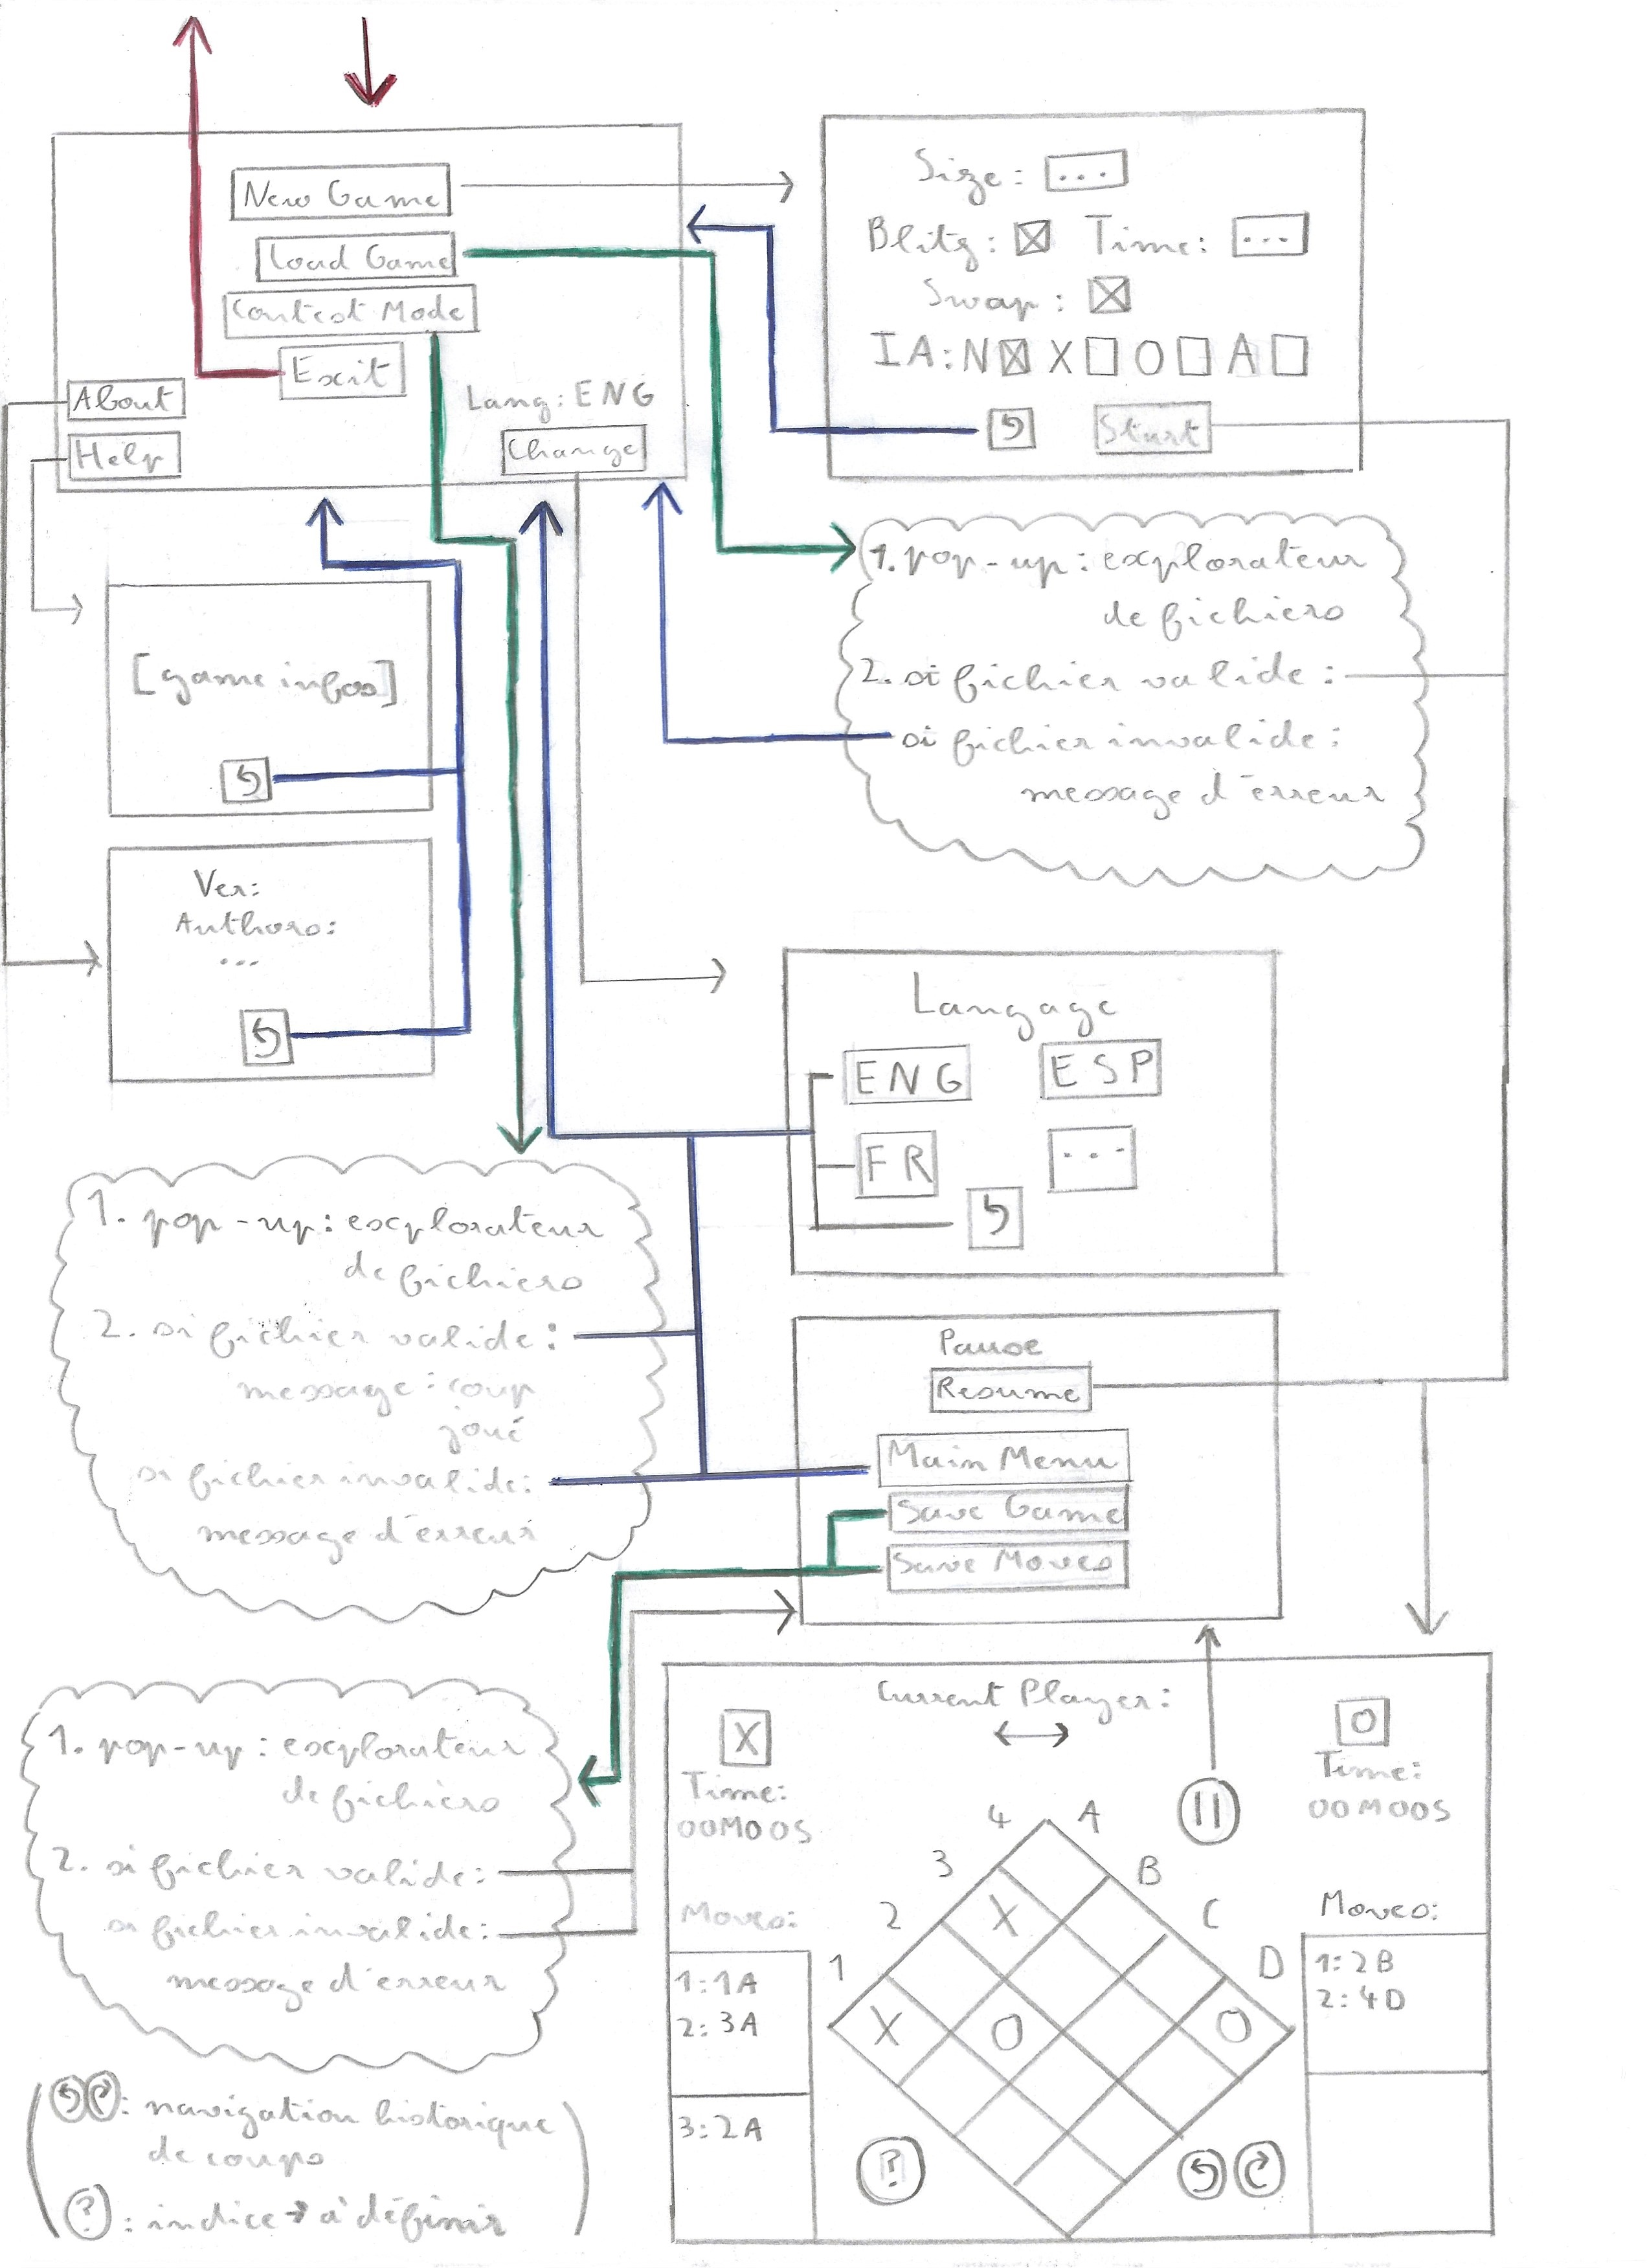
\includegraphics[width=0.75\linewidth]{GUI.jpg}
    \label{fig:GUI}
\end{figure}

\medskip
\begin{itemize}
    \item \textbf{F46 :} Menu "File"
    \begin{itemize}
        \item \textbf{Besoin fonctionnel}
        \item \textbf{Description :} L’interface graphique devra comporter un menu principal qui permettra de lancer une nouvelle partie (’New Game’), de charger une partie depuis un fichier (’Load Game’), de sauvegarder la partie en cours dans un fichier (’Save Game’), de quitter le programme (’Quit’), d’afficher l’aide (’Help’) ou d'éditer la configuration par défaut (’Settings’).
        \item \textbf{Sous-besoin(s) :}
        \begin{itemize}
            \smallskip
            \item \textbf{F46.1 :} Nouvelle partie
            \begin{itemize}
                \item \textbf{Besoin fonctionnel}
                \item \textbf{Description :} Permettr de créer une nouvelle partie via un menu du GUI.
                 \item \textbf{Prérequis :} Réglages du jeu (\textbf{F51}).
                 \item \textbf{Actions :} Dans le menu principal, un bouton doit être ajouté qui redirige vers un menu de sélection des paramètres du jeu (\textbf{F51}) avant de pouvoir lancer la partie.
                 \item \textbf{Tests :} Tester l'existence ou les valeurs des widgets associés à cette fonctionnalité via un scénario prédéfini.
            \end{itemize}
            \smallskip
            \item \textbf{F46.2 :} Charger une partie
            \begin{itemize}
                \item \textbf{Besoin fonctionnel}
                \item \textbf{Description :} Charger une partie depuis l'interface graphique.
                \item \textbf{Prérequis :} Format de fichier (\textbf{F39}).
                \item \textbf{Actions :} Créer un bouton de chargement de partie sur le menu principal. Lorsque l’utilisateur clique sur ce bouton, un explorateur de fichier s’ouvre avec lequel l’utilisateur renseigne le fichier à charger. Une alerte d’erreur s’affiche s'il y a une erreur de lecture du fichier.
                \item \textbf{Tests :} Tester l'existence ou les valeurs des widgets associés à cette fonctionnalité via un scénario prédéfini.
            \end{itemize}
            \smallskip
            \item \textbf{F46.3 :} Sauvegarder une partie
            \begin{itemize}
                \item \textbf{Besoin fonctionnel}
                \item \textbf{Description :} Pouvoir sauvegarder une partie en cours via l'interface graphique. 
                \item \textbf{Prérequis :} Sauvegarder une partie (\textbf{F33.2}), Affichage d'une partie en cours (\textbf{F46}).
                \item \textbf{Actions :} Depuis une partie en cours, il doit être possible de sélectionner un bouton (possiblement via un menu de pause) qui permette de sauvegarder la partie courante dans un fichier.
                \item \textbf{Tests :} Tester l'existence ou les valeurs des widgets associés à cette fonctionnalité via un scénario prédéfini.
            \end{itemize}
            \smallskip
            \item \textbf{F46.4 :} Quitter
            \begin{itemize}
                \item \textbf{Besoin fonctionnel}
                \item \textbf{Description :} Permettre de quitter le jeu depuis l'interface graphique.
                \item \textbf{Prérequis :} Quitter le jeu (\textbf{F33}).
                \item \textbf{Actions :} Depuis le menu principal, un bouton doit servir à quitter le jeu en appelant la fin du programme lorsque sélectionné.
                \item \textbf{Tests :} Tester l'existence ou les valeurs des widgets associés à cette fonctionnalité via un scénario prédéfini.
            \end{itemize}
            \smallskip
            \item \textbf{F46.5 :} Aide
            \begin{itemize}
                \item \textbf{Besoin fonctionnel}
                \item \textbf{Description :} Permette à l’utilisateur de consulter les règles du jeu, l’objectif ainsi que les fonctionnalités disponibles dans l’interface graphique.
                \item \textbf{Actions :} Depuis le menu principal, il doit être possible de voir l'aide du jeu via un bouton qui redirige vers une fenêtre spécifique, cette dernière comportant un bouton de retour vers le menu principal.
                \item \textbf{Tests :} Tester l'existence ou les valeurs des widgets associés à cette fonctionnalité via un scénario prédéfini.
            \end{itemize}
        \end{itemize}
    \end{itemize}
\bigskip
    \item \textbf{F47 :} Interface de jeu
    \begin{itemize}
        \item \textbf{Besoin fonctionnel}
        \item \textbf{Description :} L’interface graphique devra comporter un menu de jeu qui permettra de demander un conseil (’Hint’), naviguer dans l’historique (revenir en arrière, aller en avant, etc).
        \item \textbf{Prérequis :} Lancer l’interface graphique (\textbf{F27}), Fonctions de base GUI (\textbf{F45})
        \item \textbf{Sous-besoin(s) :}
        \begin{itemize}
            \smallskip
            \item \textbf{F47.1 :} Item Hint
            \begin{itemize}
                \item \textbf{Besoin fonctionnel}
                \item \textbf{Description :} L'interface de jeu devra comporter un item qui permet au joueur de demander un conseil (’Hint’).
                \item \textbf{Prérequis :} Affichage d'une partie en cours (\textbf{F46}).
                \item \textbf{Actions :} Sur l’affichage de la partie en cours, ajouter un bouton qui permettre aux joueurs d'obtenir un conseil de jeu.
                \item \textbf{Tests :} Tester l'existence ou les valeurs des widgets associés à cette fonctionnalité via un scénario prédéfini.
            \end{itemize}
            \smallskip
            \item \textbf{F47.2 :} Items pour l’historique
            \begin{itemize}
                \item \textbf{Besoin fonctionnel}
                \item \textbf{Description :} L'interface de jeu devra comporter des widgets permettant aux joueurs de naviguer dans l'historique.
                \item \textbf{Prérequis :} Historique de coups (\textbf{F35}), Affichage d'une partie en cours (\textbf{F46}).
                \item \textbf{Actions :} Depuis une partie en cours, ajouter deux boutons qui permettent d'annuler un coup et de rejouer un coup annulé en se servant des fonctions de l'historique des coups. 
                \item \textbf{Tests :} Tester l'existence ou les valeurs des widgets associés à cette fonctionnalité via un scénario prédéfini.
            \end{itemize}
            \smallskip
            \item \textbf{F47.3 :} Item Abandon
            \begin{itemize}
                \item \textbf{Besoin fonctionnel}
                \item \textbf{Description :} L’interface de jeu devra un item avoir ‘give up’ qui permette au joueur d’abandonner la partie en cours.
                \item \textbf{Prérequis :} Abandon (\textbf{F31})
                \item \textbf{Actions :} Sur l'affichage d'une partie en cours, ajouter un bouton qui permette d'abandonner la partie en revenant au menu principal (possiblement via un menu de pause).
                \item \textbf{Tests :} Tester l'existence ou les valeurs des widgets associés à cette fonctionnalité via un scénario prédéfini.
            \end{itemize}
        \end{itemize}
    \end{itemize}
\bigskip
    \item \textbf{F48 :} Menu "About"
    \begin{itemize}
        \item \textbf{Besoin fonctionnel}
        \item \textbf{Prérequis :} Fonctions de base GUI (\textbf{F45})
        \item \textbf{Description :} L’interface graphique devra comporter un menu d’options qui permettra de consulter des informations sur le programme (version, auteurs...).
        \item \textbf{Actions :} Sur l'affichage du menu principal, ajouter un bouton qui redirige vers une fenêtre affichant les informations voulues, avec la possibilité de revenir vers le menu principal.
        \item \textbf{Tests :} Tester l'existence ou les valeurs des widgets associés à cette fonctionnalité via un scénario prédéfini.
    \end{itemize}
\bigskip
    \item \textbf{F45 :} Fonctions de base
    \begin{itemize}
        \item \textbf{Description :} Toutes les fonctions demandées pour l’interface en console devront être implémentées dans l’interface graphique.
        \item \textbf{Prérequis :} Lancer l’interface graphique (\textbf{F27}) et PyGObject (\textbf{F12})
        \item \textbf{F45.1 :} Jouer un coup
        \begin{itemize}
            \item \textbf{Besoin fonctionnel}
            \item \textbf{Description :} Permettre à un joueur de joueur un coup depuis une partie en cours via le GUI.
            \item \textbf{Actions :} Sur l'affichage de la partie en cours, il doit être possible de cliquer sur le plateau. Cela met à jour l’affichage du plateau en "coloriant" la case choisie. Si le joueur clique sur une case déjà occupée, il ne se passe rien.
            \item \textbf{Tests :} Tester l'existence ou les valeurs des widgets associés à cette fonctionnalité via un scénario prédéfini.
        \end{itemize}
    \end{itemize}
\bigskip
    \item \textbf{F49 :} Affichage d’une partie en cours
    \begin{itemize}
        \item \textbf{Sous-besoin(s) :}
        \begin{itemize}
            \smallskip
            \item \textbf{F49.1 :} Affichage du plateau
            \begin{itemize}
                \item \textbf{Besoin fonctionnel}
                \item \textbf{Actions :} Afficher le plateau comme dans le croquis \ref{fig:GUI}.
                \item \textbf{Tests :} Tester l'existence ou les valeurs des widgets associés à cette fonctionnalité via un scénario prédéfini.
            \end{itemize}
            \textbf{}
            \item \textbf{F49.2 :} Afficher le joueur courant
            \begin{itemize}
                \item \textbf{Besoin fonctionnel}
                \item \textbf{Description :} L’interface graphique devra comporter un en-tête qui permettra de consulter le joueur courant.
                \item \textbf{Prérequis :} Fonctions de base GUI (\textbf{F45})
                \item \textbf{Actions :} Sur l'affichage de la partie en cours, ajouter un widget affichant simplement quel est le joueur en cours.
                \begin{figure}[H]
                    \centering
                    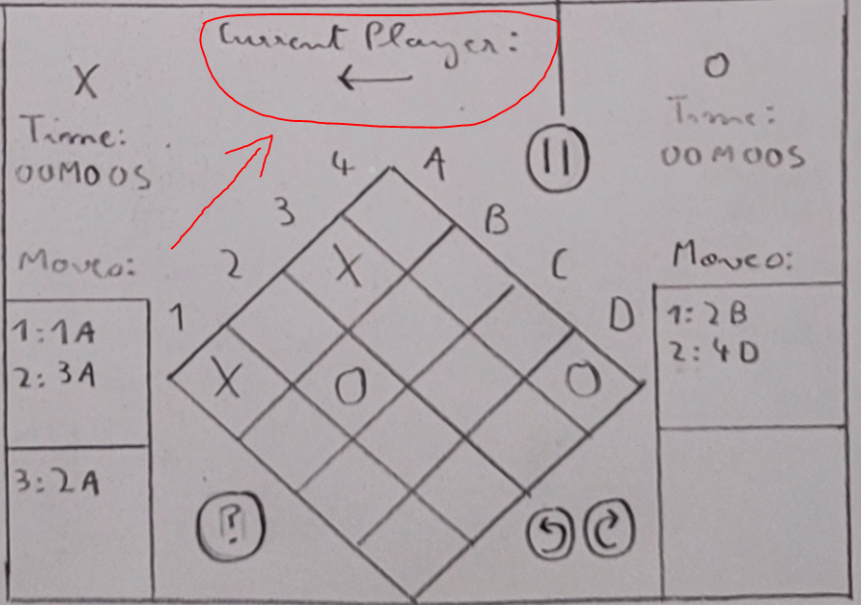
\includegraphics[width=0.5\linewidth]{gui_player.png}
                    \caption{Croquis avec l'emplacement de l'affichage du joueur entouré en rouge}
                    \label{fig:gui_player}
                \end{figure}
                \item \textbf{Tests :} Tester l'existence ou les valeurs des widgets associés à cette fonctionnalité via un scénario prédéfini.
            \end{itemize}
        \end{itemize}
    \end{itemize}
\bigskip
    \item \textbf{F50 :} Affichage des coups joués
    \begin{itemize}
        \item \textbf{Besoin fonctionnel}
        \item \textbf{Description :} L’interface graphique devra afficher sur un côté de l’interface, les coups joués lors de la partie en les numérotant.
        \item \textbf{Prérequis :} Fonctions de base GUI (\textbf{F45}), Module history (\textbf{F30.2})
        \item \textbf{Actions :} Afficher dans une liste les coups joués avec le plus récent en tête de liste.
        \begin{figure}[H]
            \centering
            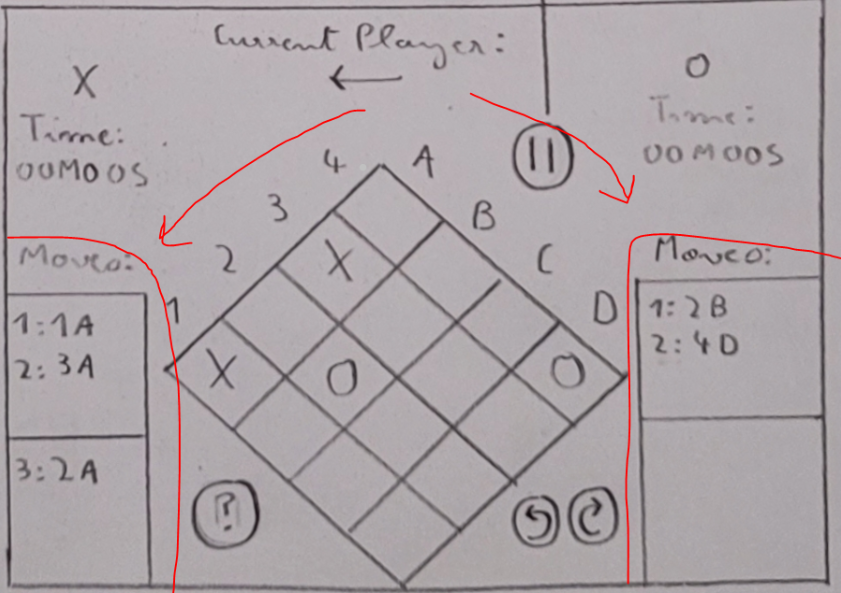
\includegraphics[width=0.5\linewidth]{gui_history.png}
            \caption{Croquis avec l'emplacement de l'affichage des coups joués entouré en rouge}
            \label{fig:gui_history}
        \end{figure}
        \item \textbf{Tests :} Tester l'existence ou les valeurs des widgets associés à cette fonctionnalité via un scénario prédéfini.
    \end{itemize}
\bigskip
    \item \textbf{F51 :} Configuration d’une nouvelle partie
    \begin{itemize}
        \item \textbf{Besoin fonctionnel}
        \item \textbf{Description :} Permettre de sélectionner les paramètres du jeu avant de lancer une partie.
        \item \textbf{Prérequis :} Toutes les options, Fichier de configuration (\textbf{F41})
        \item \textbf{Actions :} Lorsqu'une nouvelle partie est sélectionnée depuis le menu principal, il devra être possible de choisir tous les paramètres associés au jeu depuis un autre menu / fenêtre, puis de lancer la partie avec les paramêtres définis ou d'annuler et de revenir au menu principal.
        \item \textbf{Tests :} Tester l'existence ou les valeurs des widgets associés à cette fonctionnalité via un scénario prédéfini.
    \end{itemize}
\bigskip
    \item \textbf{F13 :} Module de framework d’internationalisation gettext
    \begin{itemize}
        \item \textbf{F13.3 :} Changer le langage dans le menu de l’interface graphique
        \begin{itemize}
            \item \textbf{Besoin fonctionnel}
            \item \textbf{Description :} Laisser la possibilité au joueur de changer la langue du jeu via un menu.
            \item \textbf{Prérequis :} menu principal de l’interface graphique (\textbf{F46})
            \item \textbf{Actions :} Dans le menu principal de l'interface graphique (\textbf{F27}), ajouter un bouton qui affiche un sous-menu dans lequel le joueur peut changer le langage du jeu.
            \item \textbf{Tests :} Tester l'existence ou les valeurs des widgets associés à cette fonctionnalité via un scénario prédéfini.
        \end{itemize}
    \end{itemize}
\end{itemize}

\subsubsection{Joueur Artificiel}
\medskip
\begin{itemize}
    \item \textbf{F24 :} Mode contest
    \begin{itemize}
        \item \textbf{Besoin fonctionnel}
        \item \textbf{Description :} Le mode contest doit permettre de faire s’affronter deux programmes en utilisant un fichier représentant l’état courant d’une partie.
        \item \textbf{Note :} Ne fonctionne pas si deux programmes comprennent différentes syntaxes de fichier de jeu.
        \item \textbf{Sous-besoin(s) :}
        \begin{itemize}
            \smallskip
            \item \textbf{F24.1 :} Vérification de l’option en ligne de commande
            \begin{itemize}
                \item \textbf{Prérequis :} vérification des options en ligne de commande (\textbf{F15.1}).
                \item \textbf{Actions :} À l’aide du module argparse (F11), on doit pouvoir reconnaître l’option “-c FILENAME”\\”--contest FILENAME”.
                \item \textbf{Tests :} Vérifier que le programme soit bien dans ce mode si lancé avec cette option.
            \end{itemize}
            \smallskip
            \item \textbf{F24.2 :} Mise à jour du fichier de jeu
            \begin{itemize}
                \item \textbf{Prérequis :} chargement et sauvegarde de fichier (F39), IA de jeu (F53 / F54 / F55 / F56).
                \item \textbf{Actions :} Lire le fichier FILENAME puis mettre à jour le fichier en jouant le meilleur coup en fonction du joueur courant avec une IA.
                \item \textbf{Tests :} On pourra lire le fichier après avoir joué dans ce mode sur une partie simple pour vérifier qu’un coup ait bien été joué (et vérifier s’il est “optimal”).
            \end{itemize}
        \end{itemize}
    \end{itemize}
\bigskip
    \item \textbf{F25 :} Mode IA
    \begin{itemize}
        \item \textbf{Besoin fonctionnel}
        \item \textbf{Description :} Le programme doit pouvoir être joué en mode joueur contre IA ou IA contre IA.
        \item \textbf{Prérequis :} Vérification des options spécifiées en ligne de commande (\textbf{F15.1}), Algorithme de recherche Minimax (\textbf{F53}), Heuristiques (\textbf{F52 + F59 + F58}), Monte Carlo Tree Search (\textbf{F56})
        \item \textbf{Actions :} lancer le programme, avec l’un des joueurs contrôlés par une intelligence artificielle, via l’option  “-a [COLOR]”/”--ai [=COLOR]” avec [COLOR] une valeur parmi (“X”, “O” et “A” (All), ’O’ par défaut). À l’aide du module argparse (F11), on est capable de savoir si l’option a été passée en ligne de commande. Selon la couleur passée en argument, désactiver les demandes de l’interface utilisateur pour ce joueur. Chaque coup doit être joué à l’aide de la fonction \textit{ai\_play\_move(int player)} qui retourne un coup valide basé sur l’exploration des coups faite dans un premier temps par MinMax\_tree\_search puis sera remplacée par Monte\_carlo\_tree\_search lorsque cette recherche sera implémentée.
        \item \textbf{Tests :} Vérifier qu’il n’y a aucune écriture du ou des  joueurs contrôlés par l’IA ni sur l’entrée ni sur la sortie. Ensuite, vérifier qu’à chaque tour un coup est joué par le ou les joueurs contrôlés.
    \end{itemize}
\bigskip
    \item \label{heuristique1} \textbf{F52 :} Heuristique d’évaluation de position
    \begin{itemize}
        \item \textbf{Besoin fonctionnel}
        \item \textbf{Description :} Le programme devra comporter au moins une fonction capable de prendre un état du jeu et de lui donner un score en fonction de différents critères qui vous sembleront pertinents.
        \item \textbf{Prérequis :} Plateau, Joueur courant (\textbf{F44.1})
        \item \textbf{Actions :} Implémenter une fonction \textit{evaluate(game\_state, move)} qui renvoie le score selon la configuration actuelle du plateau et un coup possible à jouer. On pourra, dans un premier temps, implémenter l’heuristique Y-réduction avec des probabilités de possession \cite{RJ02}. Le principe est d’utiliser la structure obtenue avec la réduction, mais, à la place de pairs de bits pour le codage, les cases vides sont représentées par une probabilité $p_1 = 0.5$, les cases possédées par Ami ont une probabilité $p_2$ = 1 et les cases possédées par Ennemi ont une probabilité $p_3 = 0$. Pour chaque triplet, la nouvelle opération est $q = 1/2 (p1 + p2 + p3 - p1p2p3)$. L’évaluation finale d’un coup est : $\frac{\partial v}{\partial q}.\frac{1}{2}(1-p_2p_3)$
        \item \textbf{Tests :} Vérifier la valeur de certaines configurations de plateau. Comparer le résultat, pour les 2 joueurs, d’un nœud avantageux pour un joueur.
    \end{itemize}
\bigskip
    \item \label{minimax} \textbf{F53 :} Algorithme de recherche Minimax
    \begin{itemize}
        \item \textbf{Besoin fonctionnel}
        \item \textbf{Description :} Le choix du meilleur coup se fera via une exploration de l’arbre des coups possibles via l’algorithme de recherche Minimax. Cette option sera activée par défaut si le programme est lancé en mode joueur artificiel.
        \item \textbf{Prérequis :} Heuristiques (\textbf{F52, F59}), Profondeur de recherche (\textbf{F57})
        \item \textbf{Actions :} Implémenter une fonction \textit{MinMax\_tree\_search(board, depth, current\_player)} qui prend en entrée l’état du jeu, la profondeur maximale et le joueur courant utilisant l’algorithme Minimax. Elle explore l’arbre des coups possibles jusqu’à une certaine profondeur, utilise la fonction \textit{evaluate} sur les feuilles et renvoie le coup qui permet d’avancer dans la branche contenant la feuille avec le score le plus élevé.
        \item \textbf{Tests :} Tester sur des scénarios prédéfinis de profondeurs croissantes. Par exemple, on fournit un plateau où il ne reste qu’un coup pour gagner la partie. Un autre exemple serait un plateau avec lequel le joueur doit bloquer la progression de l’autre joueur sinon il va perdre.
    \end{itemize}
\bigskip
    \item \label{alphabeta} \textbf{F54 :} $\alpha\beta$-pruning
    \begin{itemize}
        \item \textbf{Besoin fonctionnel}
        \item \textbf{Description :} L’option ’–-ai-mode ab ’ remplacera l’algorithme d’exploration par défaut par un algorithme de $\alpha\beta$-pruning
        \item \textbf{Sous-besoin(s) :}
        \begin{itemize}
            \smallskip
            \item  \textbf{F54.1 :} Option ai-mode ab
            \begin{itemize}
                \item \textbf{Prérequis :} Vérification des options spécifiées en ligne de commande (\textbf{F15.1})
                \item \textbf{Actions :} Ajouter l’option avec argparse.
                \item \textbf{Tests :} Vérifier que la fonction alphabeta est appelée lorsque cette option est passée en argument du programme et qu’elle n’est pas appelée sinon.
            \end{itemize}
            \smallskip
            \item \textbf{F54.2 :} Recherche avec $\alpha\beta$-pruning
            \begin{itemize}
                \item \textbf{Prérequis :} Heuristiques (\textbf{F52, F59}), Profondeur de recherche (\textbf{F57})
                \item \textbf{Actions :} Implémenter une fonction \textit{alphabeta(board, depth, current\_player, alpha, beta)} qui reprend l’algorithme Minimax en ajoutant l’élagage alphabeta. Les évaluations sont faites au niveau des feuilles. Si on est sur un nœud Ami, on prend la valeur maximale entre le score et alpha, Si on est sur un nœud Ennemi, on prend la valeur minimale entre le score et beta. Si alpha >= beta on peut élaguer les sous-arbres du nœud actuel.
                \item \textbf{Tests :} Cet algorithme est censé avoir les mêmes résultats que MiniMax. On doit donc comparer leur résultat sur les mêmes scénarios prédéfinis et sur un scénario aléatoire.
            \end{itemize}
        \end{itemize}
    \end{itemize}
\bigskip
    \item \textbf{F55 :} Exploration peu profonde préliminaire
    \begin{itemize}
        \item \textbf{Besoin fonctionnel}
        \item \textbf{Description :} L’option ’–-ai-shallow’ permettra d’activer une exploration préliminaire peu profonde de l’arbre des coups possibles, puis d’ordonner les coups en fonction de leur intérêt, ceci pour tirer le maximum de profit de l’$\alpha\beta$-pruning.
        \item \textbf{Sous-besoin(s) :}
        \begin{itemize}
            \smallskip
            \item \textbf{F55.1 Option ai-shallow}
            \begin{itemize}
                \item \textbf{Prérequis :} Vérification des options spécifiées en ligne de commande (\textbf{F15.1})
                \item \textbf{Actions :} Ajouter l’option avec argparse. Rajouter un paramètre booléen \textit{shallow\_exploration} à la fonction alphabeta qui par défaut est égale à False.
                \item \textbf{Tests :} Vérifier que la fonction alphabeta est appelée avec \textit{shallow\_exploration} égal à True lorsque cette option est passée en argument du programme et qu’il est égal à False sinon.
            \end{itemize}
            \smallskip
            \item \textbf{F55.2 :} $\alpha\beta$-pruning avec exploration préliminaire
            \begin{itemize}
                \item \textbf{Prérequis :} $\alpha\beta$-pruning (\textbf{F54})
                \item \textbf{Actions :} Si \textit{shallow\_exploration} est égal à True, à chaque fois que l’on génère la liste des coups possibles, on applique la fonction \textit{evaluate} sur le nœud correspondant à chaque coup possible. On trie ensuite les coups possibles selon leur score. Cela permet à l’algorithme \textit{alphabeta} d’élaguer plus souvent et permet, dans certains cas, de meilleures performances.
                \item \textbf{Tests :} Vérifier sur un arbre des coups possibles dont le meilleur coup se trouve en dernière position. Avec \textit{shallow\_exploration}, ce coup se retrouve dans les premiers de la liste, permet d’élaguer une majeure partie des branches et permet de gagner en performances. On peut donc tester le gain de performance en vérifiant que la différence time.time se trouve dans un certain intervalle de temps.
            \end{itemize}
        \end{itemize} 
    \end{itemize}
\bigskip
    \item \label{MonteCarlo} \textbf{F56 :} Monte Carlo Tree Search
    \begin{itemize}
        \item \textbf{Besoin fonctionnel}
        \item \textbf{Description :} L’option ’–-ai-mode mcts’ remplacera l’algorithme d’exploration par défaut par un algorithme de Monte Carlo Tree Search (MCTS). Cet algorithme prend en entrée l’état courant du jeu et, va effectuer de multiples simulations, peut contraindre en fonction du temps de réponse, par exemple, 3 secondes, c'est-à-dire que l’algo fait le plus de simulation et de calcul possible, et rend sa meilleure réponse au bout de 3 secondes, l’alternative est de limiter le nombre de simulations, l’algo renvoie la meilleure réponse obtenue au bout de 1000 simulations par exemple.
        Une simulation consiste en une suite aléatoire de coups, une fois la partie arrivée à terme (on parle de la simulation), on regarde le résultat, et on le propage au nœud précédent de l’arbre. Pour définir quel coup va être joué, on utilise la formule suivante $\frac{w_i}{n_i} + c \sqrt{\frac{\ln N_i}{n_i}}$ \cite{10.1007/11871842_29}, avec : $w_i$ le nombre de victoires simulées après le ième coup ; $n_i$ le nombre de parties simulées après le ième coup ; $c$ le paramètre d’exploration (il est choisi de manière empirique) ; $N_i$ le nombre de simulations effectuées par le parent du ième coup.
        On renvoie alors le coup avec le score le plus élevé.
        \item \textbf{Sous-besoin(s) :}
        \begin{itemize}
            \smallskip
            \item \textbf{F56.1 Option ai-mode mcts}
            \begin{itemize}
                \item \textbf{Prérequis :} Vérification des options spécifiées en ligne de commande (\textbf{F15.1})
                \item \textbf{Actions :} Utiliser time.time à chaque nœud et, si le temps est dépassé, renvoyer le meilleur coup obtenu depuis l’exploration en cours.
                \item \textbf{Tests :} Vérifier sur chaque recherche qu’après un certain temps (Un intervalle de temps ou de cycle d’horloges pour prendre en compte les fluctuations), ces recherches renvoient un coup.
            \end{itemize}
            \smallskip
            \item \textbf{F56.2 Fonction MCTS}
            \begin{itemize}
                \item \textbf{Prérequis :} Heuristiques (\textbf{F52, F59}), Profondeur de recherche (\textbf{F57})
                \item \textbf{Actions :} Implémenter la fonction \textit{monte\_carlo\_tree\_search(board, player, time\_limit)}.
                \item \textbf{Tests :} Vérifier avec un plateau aléatoire qu'un résultat correct est renvoyé après time\_limit.
            \end{itemize}
        \end{itemize}
    \end{itemize}
\bigskip
    \item \textbf{F57 :} Profondeur de recherche
    \begin{itemize}
        \item \textbf{Besoin fonctionnel}
        \item \textbf{Description :} L’option ’–-ai-depth DEPTH’ permettra de spécifier la profondeur de recherche de l’algorithme de recherche. 
        \item \textbf{Prérequis :} Vérification des options spécifiées en ligne de commande (\textbf{F15.1})
        \item \textbf{Actions :} Ajouter l’option avec argparse.
        \item \textbf{Tests :} Vérifier que le paramètre depth des fonctions de recherche du meilleur coup est bien égale à ce qui est passée en argument du programme.
    \end{itemize}
\bigskip
    \item \label{heuristique2} \textbf{F58 :} Choix des heuristiques
    \begin{itemize}
        \item \textbf{Besoin fonctionnel}
        \item \textbf{Description :} Il doit être possible de gérer plusieurs heuristiques d’évaluation de position. L’option ’–-ai-heuristic HEURISTIC’ permettra de spécifier l’heuristique choisie.
        \item \textbf{Sous-besoin(s) :}
        \begin{itemize}
            \smallskip
            \item \textbf{F58.1 Option ai-heuristic}
            \begin{itemize}
                \item \textbf{Prérequis :} Vérification des options spécifiées en ligne de commande (\textbf{F15.1})
                \item \textbf{Actions :} Récupérer l’option avec argparse. Si l’option est passée sans spécifier l’heuristique à utiliser, renvoyer une erreur et afficher la liste des heuristiques disponibles.
                \item \textbf{Tests :} Vérifier que l’heuristique spécifiée en paramètre est appelée si l’option est passée en argument du programme.
            \end{itemize}
            \smallskip
            \item \textbf{F58.2 Nouvelle heuristique}
            \begin{itemize}
                \item \textbf{Description :} On va utiliser l’algorithme de two-distance qui repose sur le fait de prendre le second meilleur chemin pour relier deux points, on part donc du fait que notre adversaire va bloquer le meilleur chemin possible. L’objectif va être de trouver la position inoccupée la plus à même de relier les deux bords du plateau. L’heuristique va donc calculer le potentiel de chaque joueur, un potentiel est défini par la plus petite distance calculée par l’algorithme de two-distance, pour les pièces d’un joueur. \\
                La formule de l’heuristique sera donc $e = M(p_B-p_W) - (a_B-a_W)$ où $p_B$ est le potentiel du joueur noir, $p_W$ est le potentiel du joueur blanc, $a_W$ est la flexibilité de l’attaque du joueur blanc, $a_B$ la flexibilité de l’attaque du joueur noir et $M$ est un grand nombre choisit de manière empirique. \\
                La flexibilité de l’attaque se définit par le nombre de pièces ayant la valeur du potentiel minimum d’un joueur.
                Si $M$ est suffisamment grand, l’heuristique va préférer un coup à un autre, et la flexibilité pourra alors servir uniquement à départager deux plateaux ayant le même potentiel. Sachant que le potentiel d’une position est fini, il ne peut dépasser $2n^2$ ($n$ largeur d’un côté), donc un $M$ autour de $n^2$, est pertinent, on utilise donc, pour un tableau de taille 11x11, $M$ = 121.
                \item \textbf{Prérequis :} Plateau, Joueur courant (\textbf{F44.1})
                \item \textbf{Actions :} Implémenter la fonction \textit{(int,int) get\_potential\_and\_mobility(int joueur)} et implémenter la fonction \textit{int two\_distance\_evaluation(int joueur)}.
                \item \textbf{Tests :} 
            \end{itemize} 
        \end{itemize}
    \end{itemize}
\bigskip
    \item \textbf{F59 :} Heuristique de fin de partie
    \begin{itemize}
        \item \textbf{Besoin fonctionnel}
        \item \textbf{Description :} Créer au moins une heuristique de fin de partie pour optimiser l’évaluation des positions.
        \item \textbf{Actions :} Dans chaque heuristique, ajouter une condition telle que si le nœud actuel correspond à la fin de partie, un score élevé est renvoyé si le plateau est gagnant et inversement si le plateau est perdant.
        \item \textbf{Tests :} Vérifier que chaque heuristique renvoie la bonne valeur sur un nœud correspondant à un plateau gagnant, un plateau perdant et un plateau quelconque.
    \end{itemize}
\mbox{}
    \item \textbf{F60 :} Temps de réflexion borné
    \begin{itemize}
        \item \textbf{Besoin fonctionnel}
        \item \textbf{Description :} L’option ’–-ai-time TIME’ permettra de spécifier le temps de réflexion de l’algorithme de recherche. Si le temps est écoulé, le programme devra jouer le meilleur coup trouvé jusqu’à présent. Par défaut, le temps de réflexion sera de 5 secondes.
        \item \textbf{Prérequis :} Vérification des options spécifiées en ligne de commande (\textbf{F15.1})
        \item \textbf{Actions :} Utiliser time.time à chaque nœud et, si le temps est dépassé, renvoyer le meilleur coup obtenu depuis l’exploration en cours.
        \item \textbf{Tests :} Vérifier sur chaque recherche qu’après un certain temps (Un intervalle de temps ou de cycle d’horloges pour prendre en compte les fluctuations), ces recherches renvoient un coup.
    \end{itemize}
\end{itemize}

\newpage
\section{Graphe des dépendances des besoins}

Les spécifications étendues des besoins nous permettent de lier les besoins entre eux par dépendances, ce qui donne le graphe \ref{fig:graph}.

\begin{figure}[H]
    \centering
    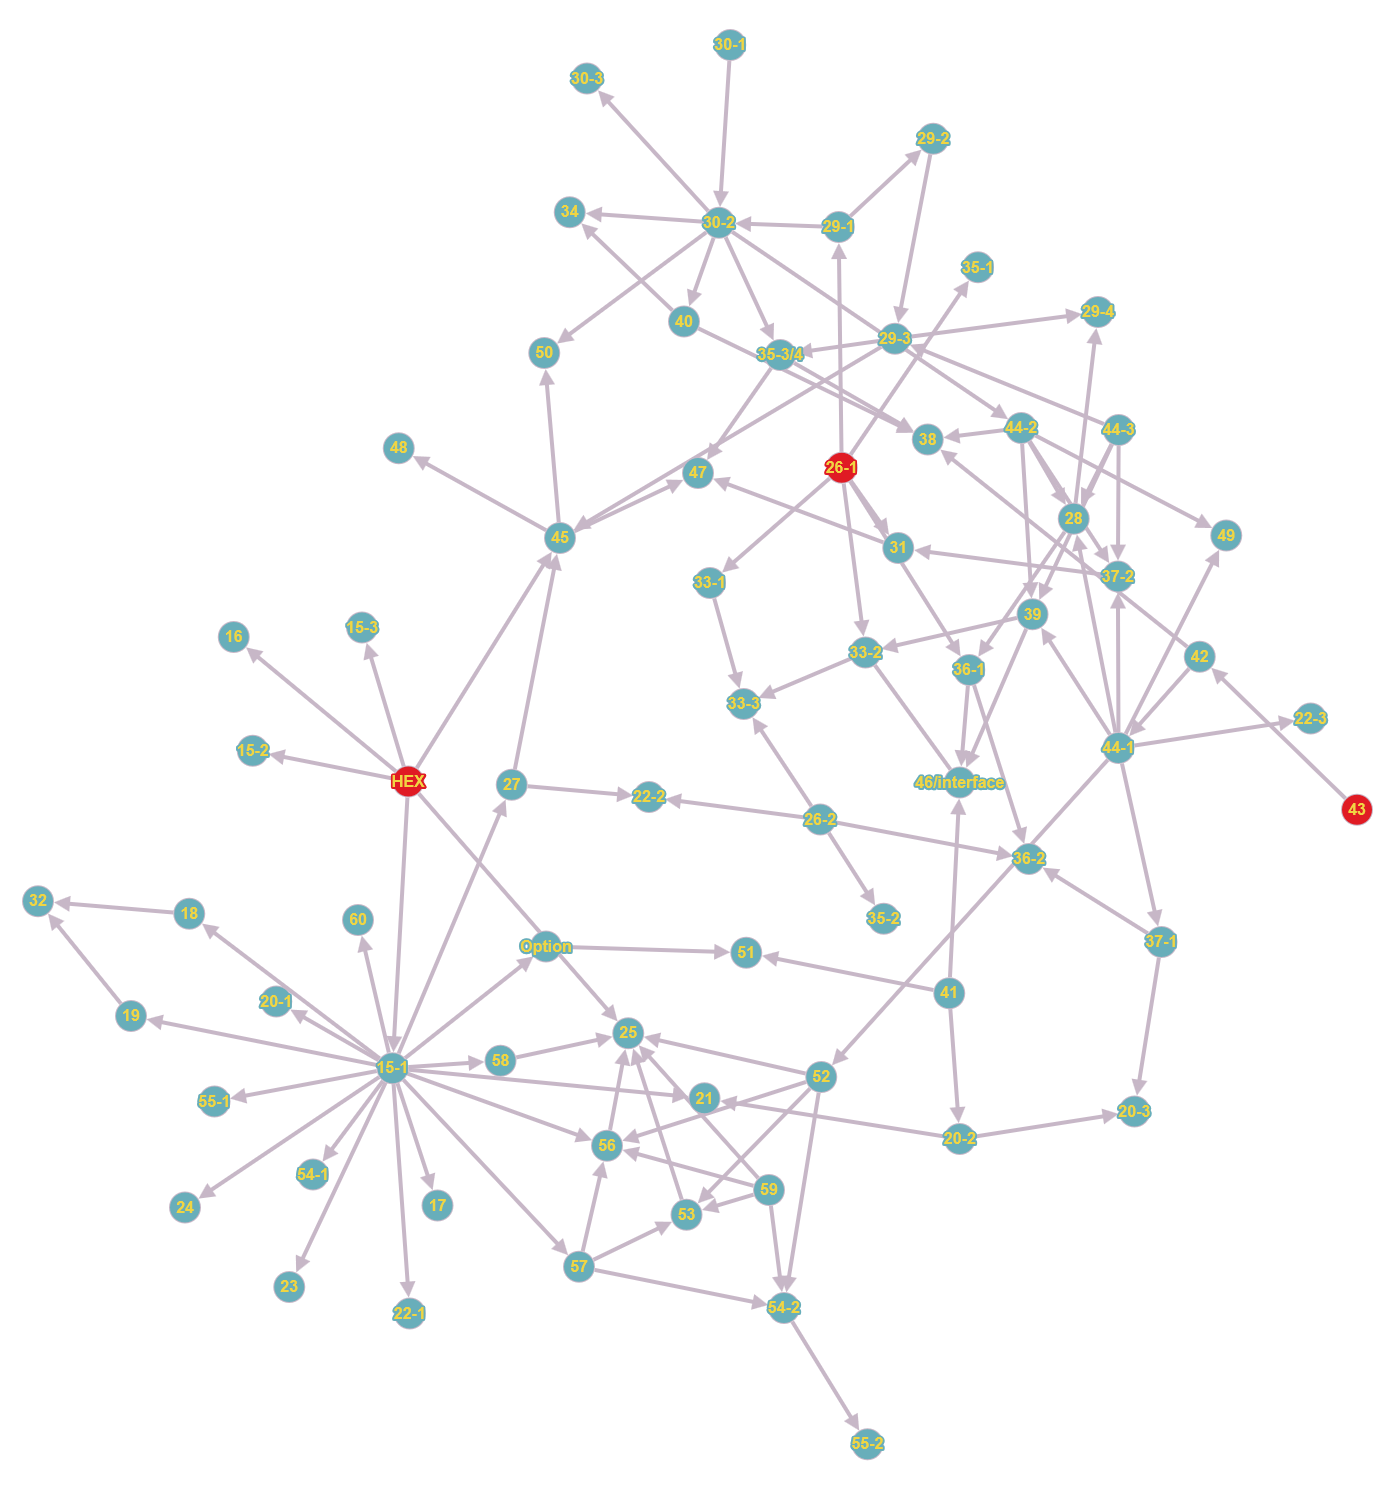
\includegraphics[width=0.75\linewidth]{graph.png}
     \caption{Graphique des dépendances de nos besoins. (En rouge, les besoins d'où on peut commencer)}
     \label{fig:graph}
\end{figure}

\newpage
\section{Diagramme de Gantt}

En se servant du graphe des dépendances, nous pouvons facilement visualiser le déroulement chronologique de projet. Nous pouvons donc créer le diagramme de Gantt (Figure \ref{fig:Gantt}). Les tâches sont réparties par semaine et non selon des dépendances. On part du principe que l'ensemble des tâches d'une même semaine peuvent être effectuées plus ou moins en même temps et nécessitent une validation rigoureuse avant la fin de la semaine.
\begin{figure}[H]
    \centering
    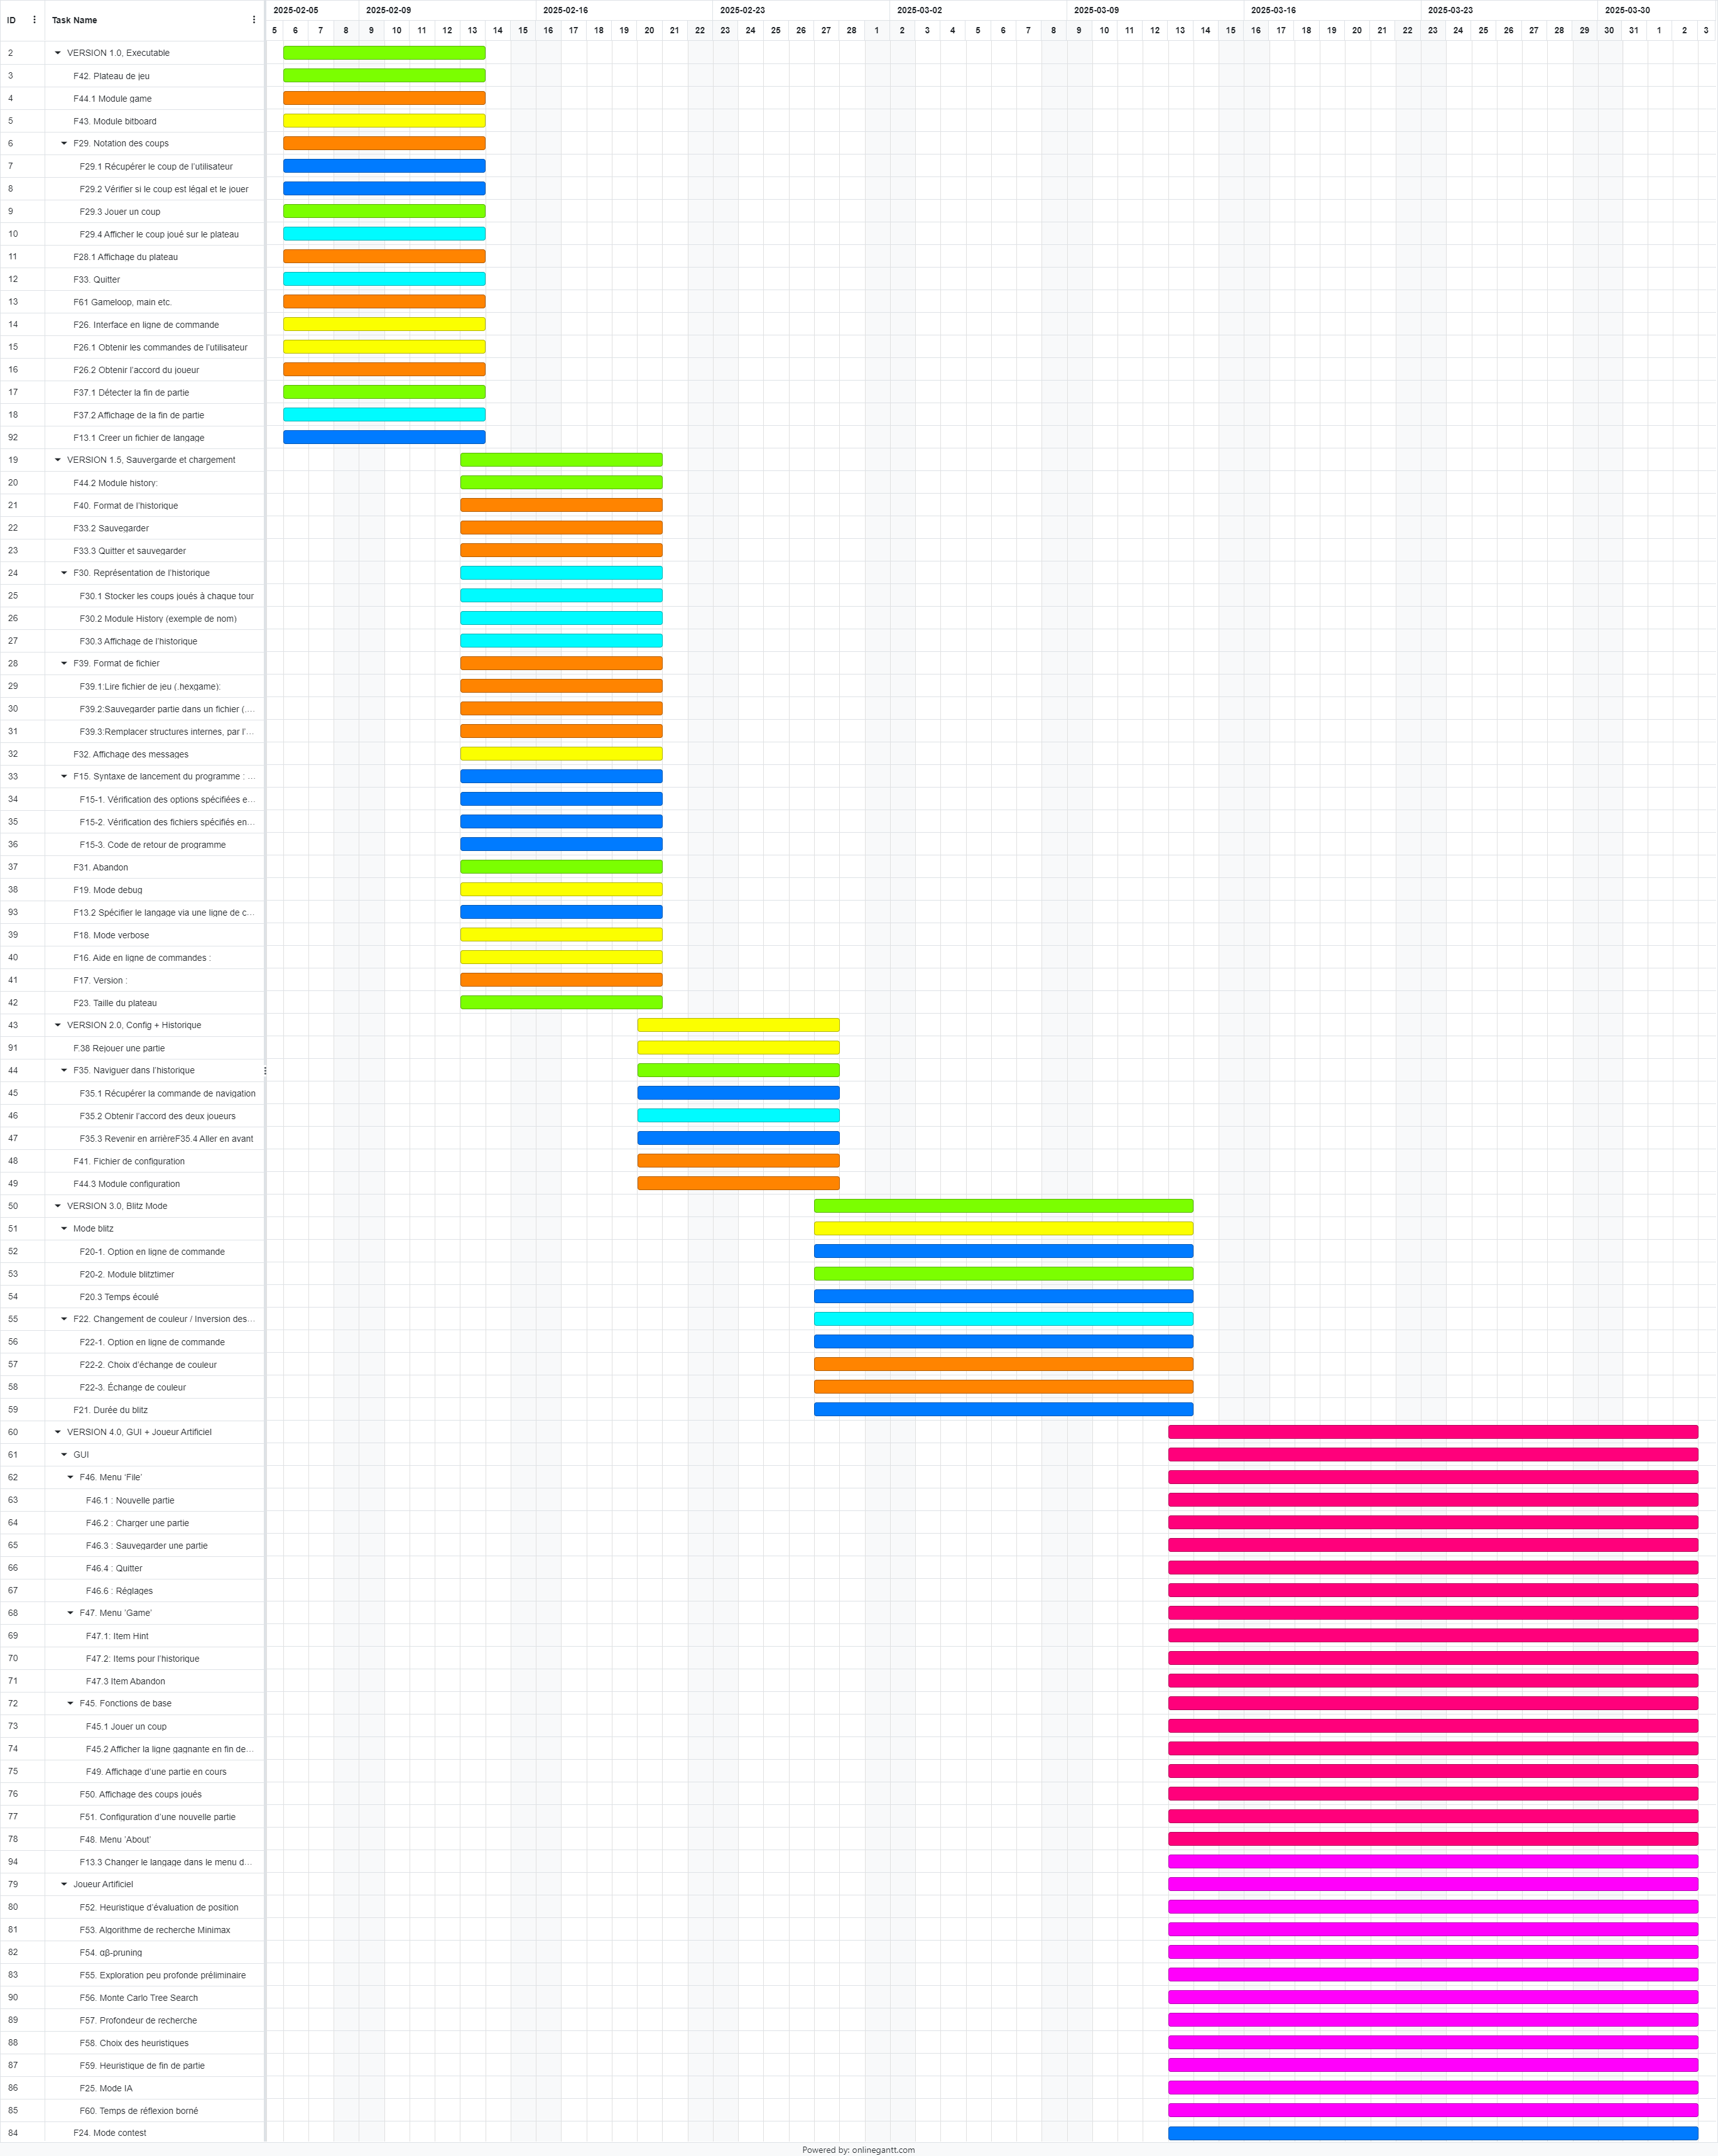
\includegraphics[width=.95\linewidth]{Gantt.png}
    \caption{Diagramme de Gantt à priori de notre projet. (en vert, KUSTERS Timon; en cyan, GUITARD Paul; en jaune ROCHETEAU Yohann; en bleu, HUBINCU Morgan; en orange, HERR Mariano; en Rouge/Rose, l'équipe GUI : GUITARD Paul, ROCHETEAU Yohann et HUBINCU Morgan; en Violet, l'équipe IA : KUSTERS Timon, HERR Mariano)}
    \label{fig:Gantt}
\end{figure}

\newpage
\section{Architecture du projet}

Le schéma \ref{fig:Architecture} représente l'architecture du projet telle que nous l'imaginons à priori. Sachant que dans le fichier ai.py contient les heuristiques et les algorithmes d'exploration utilisable, il suffit pour avoir accès à de nouvelles heuristiques de rajouter des fonctions qui prennent en entrée un plateau de jeu et  qui renvoie comme les précédentes une valeur entière. Pareil pour les algorithmes d'exploration, on peut rajouter des algorithmes qui prennent en entrée un plateau, et qui renvoie un coup à jouer, pour pouvoir les utiliser au sein de tout le programme. Il suffit aussi de modifier le fichier bitboard.py par un autre fichier décrivant une structure utilisé comme plateau de jeu, donc abritant des fonctions telles que play\_move, ou check\_legal\_move, et aussi modifier la classe Board qui joue le rôle d'intermédiaire entre la classe de la structure de donnée du plateau et le reste du projet. Les diagrammes \ref{fig:starting} et \ref{fig:valide} apportent des précisions sur l'interaction entre les différentes composantes du projet.

\begin{figure}[H]
    \centering
    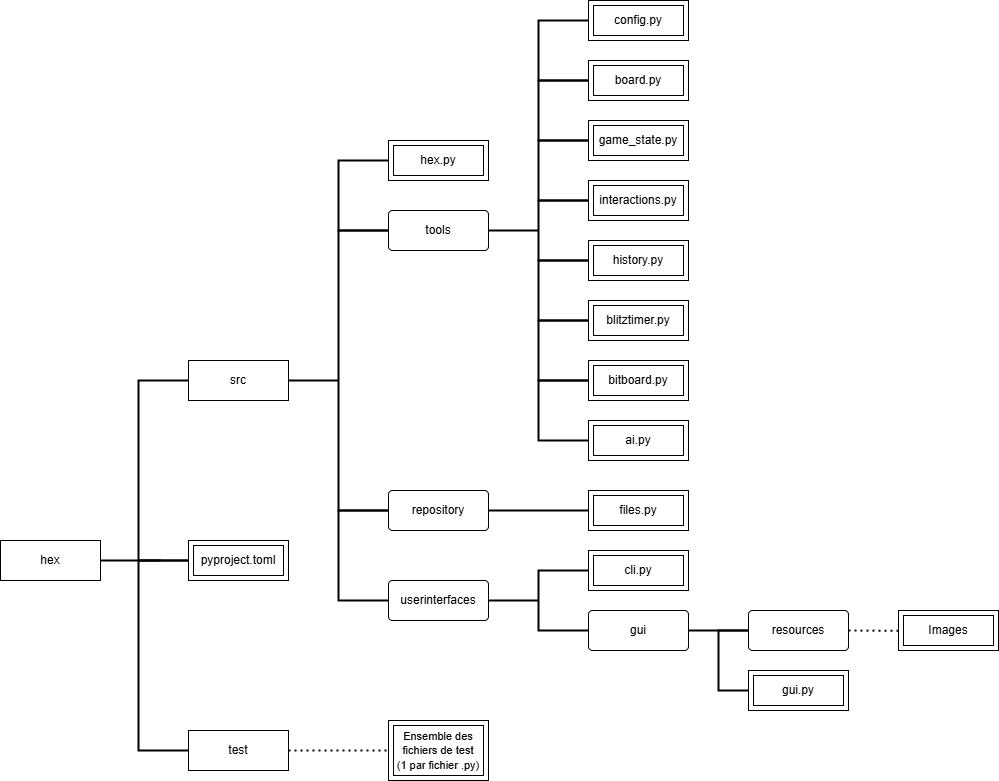
\includegraphics[width=1\linewidth]{Architecture.png}
    \caption{Architecture à priori de notre projet}
    \label{fig:Architecture}
\end{figure}

\begin{figure}[H]
    \centering
    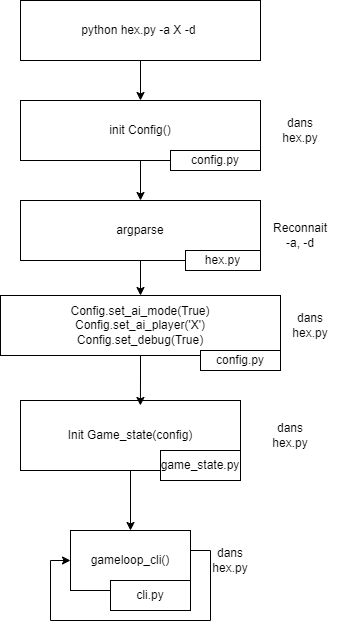
\includegraphics[width=0.4\linewidth]{Interaction_starting.png}
    \caption{Diagramme de séquence décrivant les principales fonctions appelées, lors de l'initialisation du projet}
    \label{fig:starting}
\end{figure}

\begin{figure}[H]
    \centering
    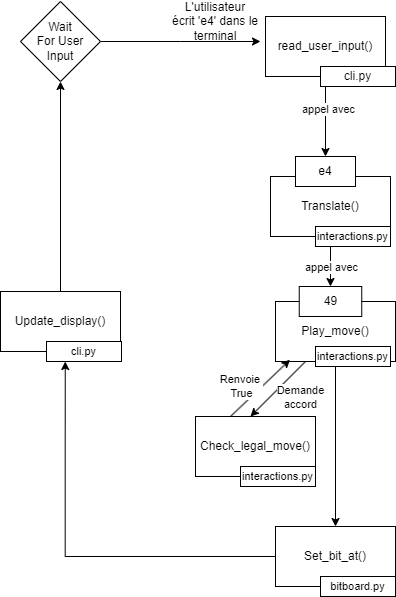
\includegraphics[width=0.4\linewidth]{Interaction_valide.png}
    \caption{Diagramme de séquence décrivant les principales fonctions appelées, lorsqu'un joueur joue un coup valide}
    \label{fig:valide}
\end{figure}

\newpage
\addcontentsline{toc}{section}{Références}
\bibliographystyle{alpha}
\bibliography{biblio}

\end{document}